\documentclass[grad,pdftex,numbers]{coppetex/coppe}
\usepackage[utf8]{inputenc}
\usepackage{amsmath,amssymb}
\usepackage{multirow}% http://ctan.org/pkg/multirow
\usepackage{hhline}% http://ctan.org/pkg/hhline
\usepackage[table,xcdraw]{xcolor}
%\usepackage{subfigure}
\usepackage{longtable}
\usepackage[portuguese]{babel}
\usepackage[linesnumbered,ruled,vlined,portugues]{algorithm2e}
\usepackage{float}
\usepackage{subfig}
%\usepackage{graphicx}
%\usepackage{caption}
\usepackage{graphicx}
%\usepackage{subcaption}

% Tabelas geradas em: http://www.tablesgenerator.com/latex_tables#

\makeloabbreviations

\begin{document}
  \title{Algoritmos para Enumeração de Conjuntos de Enlaces Viáveis em Redes Sem Fio}
  \foreigntitle{Algorithms for Enumerating Feasible Sets of Links in Wireless Networks}
  \author{Guilherme Iecker}{Ricardo}
  \advisor{Prof.}{José Ferreira}{de Rezende}{D.Sc.}
  \advisor{Prof.}{Valmir Carneiro}{Barbosa}{D.Sc.}

  \examiner{Prof.}{José Ferreira de Rezende}{D.Sc.}
  \examiner{Prof.}{Valmir Carneiro Barbosa}{D.Sc.}
  \examiner{Eng.}{Raphael de Melo Guedes}{D.Sc.}

  \department{PEE}
  \date{09}{2016}

  \keyword{Redes Sem Fio}
  \keyword{Projeto de Algoritmos}
  \keyword{Otimização Combinatória}

  \foreignkeyword{Wireless Networks}
  \foreignkeyword{Algorithms Design}
  \foreignkeyword{Combinatoric Optimization}

  \maketitle

  \frontmatter
  \chapter*{Agradecimentos}

Agradeço aos meus pais que sempre apoiaram minhas escolhas e me motivaram a alcançar meus objetivos. Agradeço também à minha irmã sempre tão amiga e companheira em todos os momentos.

Agradeço aos meus amigos Fernando, Marcel, Túlio, Paulo, Luiz Fernando, Maria Thereza, Marcella, Matheus e Lucas que trouxeram mais alegria à minha jornada, ajudando a superar os momentos difíceis.

Agradeço aos meus orientadores, Rezende e Valmir, pelas oportunidades e por compartilharem seu tempo e seu conhecimento comigo. Agradeço aos meus colegas Luiza, Priscila, Raphael e Héberte que tanto colaboraram na minha trajetória acadêmica.

Finalmente, agradeço aos meus colegas, amigos e professores do período de intercâmbio. Em especial, aos meus amigos Fábio, Moa e Daniel e aos meus orientadores, Erika, Tamara e Davi.

  Aos meus pais.

  \begin{abstract}

Rádios Cognitivos são dispositivos capazes de escutar o meio e escolher frequências disponíveis para a transmissão de dados. A escolha do canal depende da disponibilidade do mesmo. O rádio realiza uma consulta à um servidor , que retorna os canais que estão livres naquela localização. Diferentes modelos de propagação do sinal são implementados no servidor, para realização do cálculo dos canais livres. O trabalho consiste em desenvolver um servidor Web ilustrando o espectro no Estado do Rio de Janeiro, implementar um novo modelo de propagação que considere o relevo, garantir a persistência dos dados calculados anteriormente e permitir uma melhor interação do usuário com o servidor.

\end{abstract}


  \begin{foreignabstract}

Cognitive Radios are devices capable of listening to the environment and select available frequencies for data transmission. The channel choice depends on its availability. The radio makes a query to a server, which returns the channels that are available on that location. Different signal propagation models are implemented on the server, for the available channels calculation. This work aims to develop a Web server showing the spectrum in the State of Rio de Janeiro, implement a note propagation model that considers the relief, guarantee the previous data calculation and allow a better user interaction with the server.

\end{foreignabstract}

  \tableofcontents
  \listoffigures
  \listoftables
  \printloabbreviations

  \mainmatter
  \chapter{Introdução}
\label{cap:introducao}

O problema de enumeração de conjuntos de enlaces viáveis em redes sem fio surgiu de uma proposta de solução ao problema de escalonamento de enlaces. Neste capítulo, é discutido o problema de escalonamento de enlaces e como surgiu a necessidade de encontrar e listar os conjuntos de enlaces viáveis. Algumas definições importantes ao decorrer do trabalho também são apresentadas. 

Além disso, serão introduzidos a descrição formal para o problema de enumaração de conjuntos viáveis, o objetivo deste trabalho, e qual a metodologia usada para alcançá-lo. Finalmente, é descrito como o restante do texto está organizado.

\section{Motivação}

Conforme definido em \cite{mesh}, uma rede em malha sem fio, ou {\it wireless mesh network} (WMN)\abbrev{WMN}{Wireless Mesh Network}, é composta por nós que podem funcionar como {\it hosts} e roteadores simultaneamente e se comunicam diretamente através de enlaces de dados sem fio. Uma transmissão ocorre quando um nó, chamado de transmissor, envia mensagens a outro nó, chamado de receptor, através de um enlace. Em um dado período de tempo, um enlace está ativo quando há uma transmissão em curso.

Em redes sem fio que utilizam um único canal de transmissão, os nós compartilham o meio físico. Por isso, quando existe um cenário com mais de um enlace ativo, é comum que os nós transmissores de um enlace causem interferência nos nós receptores de outro enlace. Em alguns casos, essa interferência pode atrapalhar ou mesmo inviabilizar a troca de mensagens em um enlace. Portanto, faz-se necessário um mecanismo para organizar a ativação dos enlaces no tempo com o intuito de reduzir o efeito de tais interferências.

Um conjunto de enlaces ativos é dito viável quando todos os enlaces que o compõem atendem os critérios dos testes de interferência especificados em \cite{primary, sinr}. No próximo capítulo, os testes serão explicados com detalhes. Por enquanto, pode-se interpretar os testes como formas de verificar o quanto as interferências sofridas entre os enlaces de um conjunto prejudicam a comunicação.

Considerando um período de tempo T no qual diversas transmissões estão acontecendo, T pode ser particionado em um conjunto de slots de tempo $S=\{s_1, s_2, \, \ldots \, , \, s_t\}$. Conforme definido em \cite{scheduling}, o problema de escalonamento de enlaces consiste em encontrar maneiras de distribuir os enlaces ativos de uma rede em $S$, de forma que os conjuntos de enlaces em cada slot $s_i$ sejam viáveis e o número de slots seja o menor possível.

Existem diversas estratégias para resolver esse problema na literatura. Por exemplo, em \cite{scheduling}, coloração de vértices é usada para abordar o problema. Outras soluções como as descritas em \cite{dist-sched, coloring} propõem soluções no contexto de redes de sensores.

Em geral, tais estratégias baseiam-se em heurísticas que podem não apresentar os melhores resultados. Visando desenvolver um algoritmo para resolver o problema de escalonamento de enlaces e encontrar o melhor resultado, é fundamental que todos os conjuntos de enlaces viáveis sejam enumerados para serem usados como restrições de um problema de programação linear.

\section{Descrição do Problema}

Deseja-se verificar a viabilidade de todas as combinações de enlaces possíveis em uma rede em malha através de testes de interferência. O problema de enumeração de conjuntos de enlaces viáveis consiste em desenvolver um algoritmo capaz de encontrar todos os conjuntos C, tal que C é viável, com o menor tempo para que possa ser utilizado em aplicações práticas.

Caso a rede tenha $m$ enlaces, então existe um total de $2^m$ conjuntos a serem testados. Com isso, a complexidade de tempo de um algoritmo que usa força bruta pura para explorar todos os conjuntos possíveis e testar sua viabilidade é $O(2^m)$. Isto é, o tempo de excução de tal algoritmo é tão grande que torna-se impraticável utilizá-lo em aplicações reais. Se a complexidade dos testes também forem consideradas, o tempo de execução aumenta ainda mais. 

\section{Objetivo}

O objetivo deste trabalho é introduzir algoritmos baseados em força bruta que consigam resolver o problema de enumeração de conjuntos de enlaces viáveis com complexidades de tempo menores. Além disso, também será estudado o tempo real de execução dos algoritmos em diferentes cenários.
 
\section{Metodologia}

Nesse trabalho, o problema será modelado usando a ideia de árvore de combinações, que oferece propriedades fundamentais para o desenvolvimento de algoritmos com menores complexidades de tempo. Além disso, outras técnicas para otimização serão estudadas e aplicadas.

Uma vez que os algoritmos são implementados, suas eficiências serão verificadas através de experimentos em redes geradas aleatoriamente. Um estudo de como o número de conjuntos viáveis varia com o tamanho da rede será feito para avaliar as complexidades computacionais dos algoritmos. Finalmente, os tempos de execução serão avaliados.

\section{Organização do Texto}

No Capítulo~\ref{cap:modelagem}, são apresentados alguns modelos de redes de computadores e combinatória. O objetivo é estudar como reunir tais modelos para projetar algoritmos e algumas vantagens. 

Nos capítulos~\ref{cap:iterativo} e ~\ref{cap:recursivo}, os projetos dos algoritmos são apresentados. Ao final de cada capítulo, é feito uma avaliação das suas complexidades.

No capítulo~\ref{cap:resultados}, algumas técnicas de otimização adicionais são apresentadas. Depois, é feito um breve resumo das técnicas de implementação e ambientes utilizados. Conclui-se o capítulo descrevendo as simulações e analisando os resultados obtidos.

No capítulo~\ref{cap:conclusoes}, as considerações finais são feitas e alguns trabalhos decorrentes desse projeto são propostos.


  \chapter{Modelagem}
\label{cap:modelagem}

Neste capítulo, é apresentado como modelar uma rede usando grafos e como modelar as combinações de enlaces em uma árvore de combinações. 

Os modelos de iterferências são apresentados com o intuito de definir o teste de viabilidade e, futuramente, permitir algumas otimizações.

Ao final, é apresentado um exemplo de como enumerar os conjuntos viáveis ingenuamente usando os modelos introduzidos com Busca em Largura. As vantagens e desvantagens dessa abordagem são discutidas.

\section{Modelagem Redes usando Grafos}

Para modelar uma rede qualquer usando um grafo $G=(V,E)$, basta fazer as seguintes representações: Os nós da rede são os vértices do grafo, ou seja constituem o conjunto $V(G)$ e, por convenção, $|V|=n$. Os enlaces da rede são as arestas do grafo, ou seja constituem o conjunto $E(G)$ e, por convenção, $|E|=m$.

Para esse trabalho, é importante que as arestas de G sejam direcionadas já que os enlaces especificam a direção da comunicação. A Figura \ref{fig:grafo} mostra um exemplo de como tal modelagem pode ser feita para uma rede bem simples com $n=5$ e $m=4$.

\begin{figure}[htb]
\centering
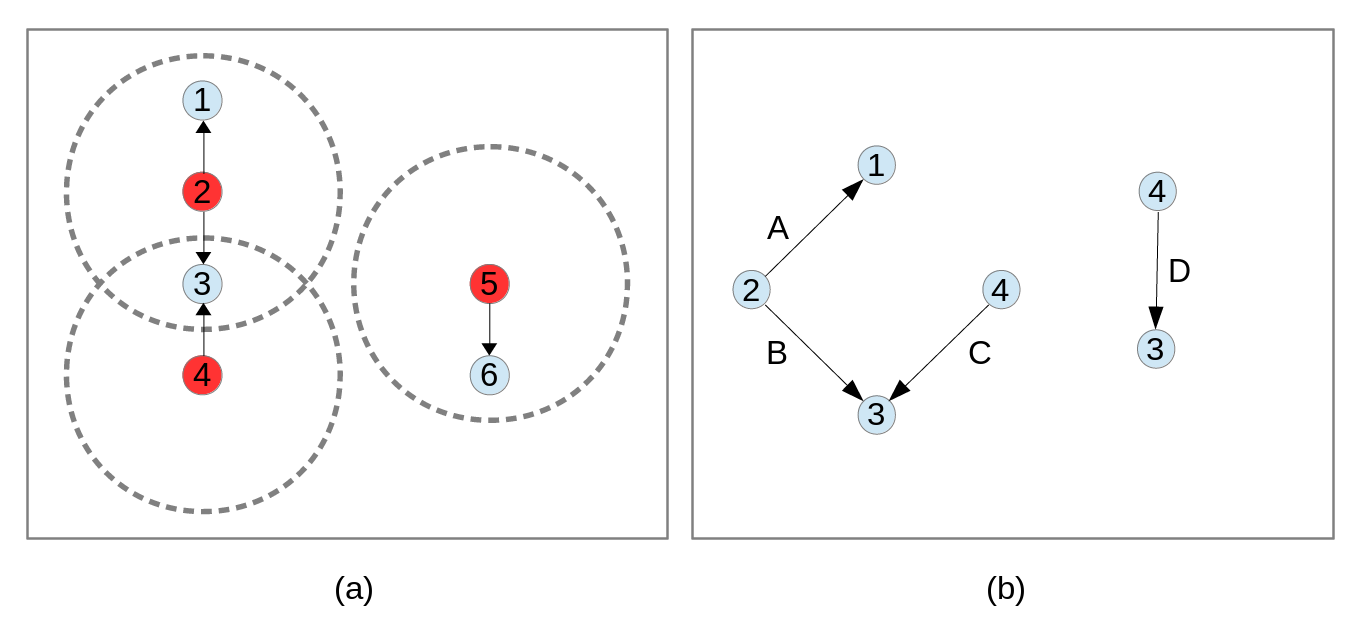
\includegraphics[width=1\textwidth]{figs/grafo}
\caption[Modelo da rede (a) usando o grafo (b).]
{Modelo da rede (a) usando o grafo (b).}
\label{fig:grafo}
\end{figure}

Modelar uma rede como um grafo é bastante útil pois permite utilizar algumas propriedades importantes da Teoria dos Grafos e fazer diversas manipulações matemáticas. Especificamente, nesse trabalho, a abstração em grafos também ajudou muito na etapa de implementação dos algoritmos.

\section{Árvore de Combinações}

Seja um grafo direcionado $G=(V,E)$. É possível definir um conjunto $C$, tal que $C \subseteq E(G)$, isto é, $C$ é uma combinação dos enlaces de $E(G)$. Com isso, tem-se que o menor tamanho de $C$ é zero, ou seja, não há enlaces ativos ($C=\emptyset$), e o maior tamanho é o próprio $E(G)$, com todos os enlaces possíveis ativos ($C=E(G)$). Entre esses dois extremos, existem $2^m$ combinações de enlaces possíveis, que são subconjuntos de $E(G)$ definidos pela escolha de quais enlaces estão ativos.

Sobre essas combinações de enlaces é possível definir uma árvore de combinações $A=(V,E)$. Os vértices da árvore são todas as combinações possíveis dos enlaces em $E(G)$. As arestas da árvore ligam qualquer combinação em uma altura $h$ a outra em uma altura $h+1$ que pode ser obtido através da adição de um enlace de $E(G)$. Em $A$, o tamanho de um vértice C a uma altura h na árvore é tal que $|C|=h$.

\begin{figure}[htb]
\centering
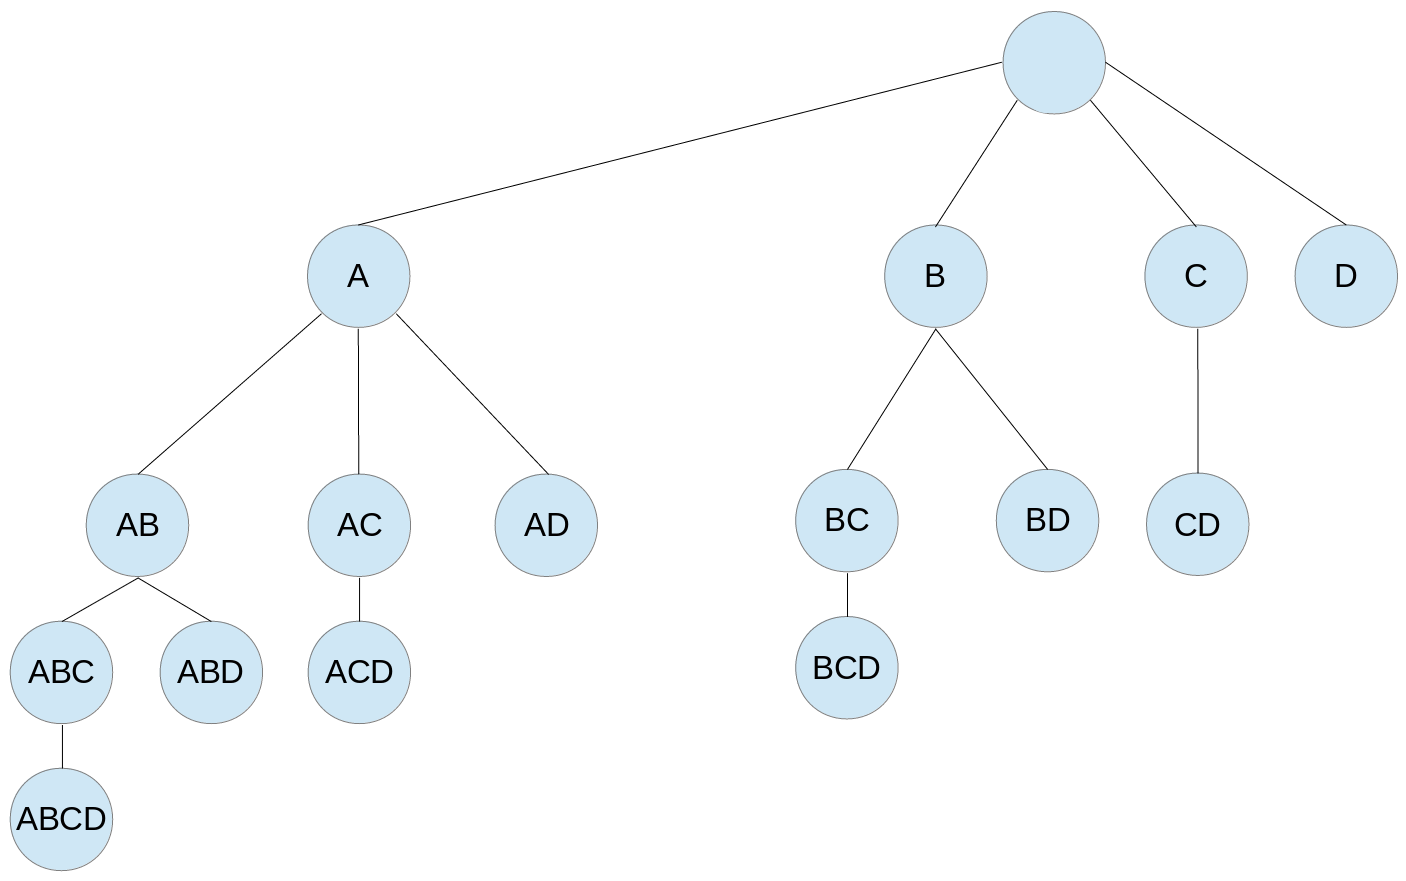
\includegraphics[width=0.7\textwidth]{figs/arvore}
\caption[Árvore de Combinações para a rede da Figura \ref{fig:grafo}.]
{Árvore de Combinações para a rede da Figura \ref{fig:grafo}.}
\label{fig:arvore}
\end{figure}

Nessa árvore, a raiz ($h=0$) é a combinação com nenhum enlace, ou seja, $C=\emptyset$ ($(|C|=0)$). Os filhos de qualquer vértice $C$ da árvore são obtidos combinando $C$ com um enlace $i \in E(G)$, tal que $i \notin C$. Para a mesma rede modelada na Figura \ref{fig:grafo}, é ilustrada sua árvore de combinações de enlaces na Figura \ref{fig:arvore}.

No contexto de árvore de combinações, é importante definir também os descendentes de um vértice. Segundo [XXX], se P(r,v) é um caminho da raiz $r$ a um vértice $v$ na árvore, $v$ é descendente de $u$ se, e somente se, $u \in P(r,v)$. 

A abstração de árvore de combinações permite que os conjuntos de enlaces sejam percorridos conforme a estrutura da árvore. Com isso, é possível desenvolver métodos sistemáticos para buscar e avaliar a viabilidade das combinações de enlaces. Os métodos mais famosos como Busca em Largura e Busca em Profundidade em árvores podem ser considerados nesse caso. Entretanto, sua utilização exige a construção prévia da árvore que apresenta alta complexidade tanto de tempo, quanto de espaço ($O(2^m)$ em ambos os casos).

Os algoritmos que serão apresentados nos próximos capítulos apenas usam a ideia de árvore de combinações em seus projetos. Não há construção da árvore para realizar buscas e isso representa uma diminuição considerável na complexidade de espaço. Além disso, eles fazem uso da propriedade apresentada na próxima seção que, por sua vez, ajuda a reduzir a complexidade de tempo.

\section{Modelos de Interferência}

No capítulo \ref{cap:introducao}, os testes de interferências foram descritos de maneira intuitiva e pouco detalhada. Nessa seção, eles serão definidos formalmente e uma propriedade decorrente da natureza desses testes será apresentada. Essa propriedade é importante pois permitirá o desenvolvimento de algoritmos de enumeração com melhores desempenhos.

Em redes sem fio, o meio físico é compartilhado. Isso significa que, apesar das mensagens geradas pelo transmissor serem destinadas um receptor específico, elas acabam atingindo todos os nós com diferentes intensidades.

\subsection{Modelo de Interferência Primária}

Na modelagem de redes sem fio, os enlaces são considerados half-duplex, isto é, os rádios dos dispositivos que compõem a rede não podem transmitir e receber mensagens ao mesmo tempo. Por isso, um nó pode apenas ser transmissor ou receptor em um dado instante de tempo.
 
\item Enlaces dedicados: Apesar das mensagens serem transmitidas em várias direções e, portanto, alcançarem diversos nós, elas são direcionadas a um nó específico. 


Ao modelar uma rede em que os enlaces possuam essas duas características, os nós apenas assumem papel de transmissor ou de receptor em, no máximo, um enlace. A figura \ref{fig:primario} ilustra essas características usando diferentes cenários.

\begin{figure}[htb]
\centering
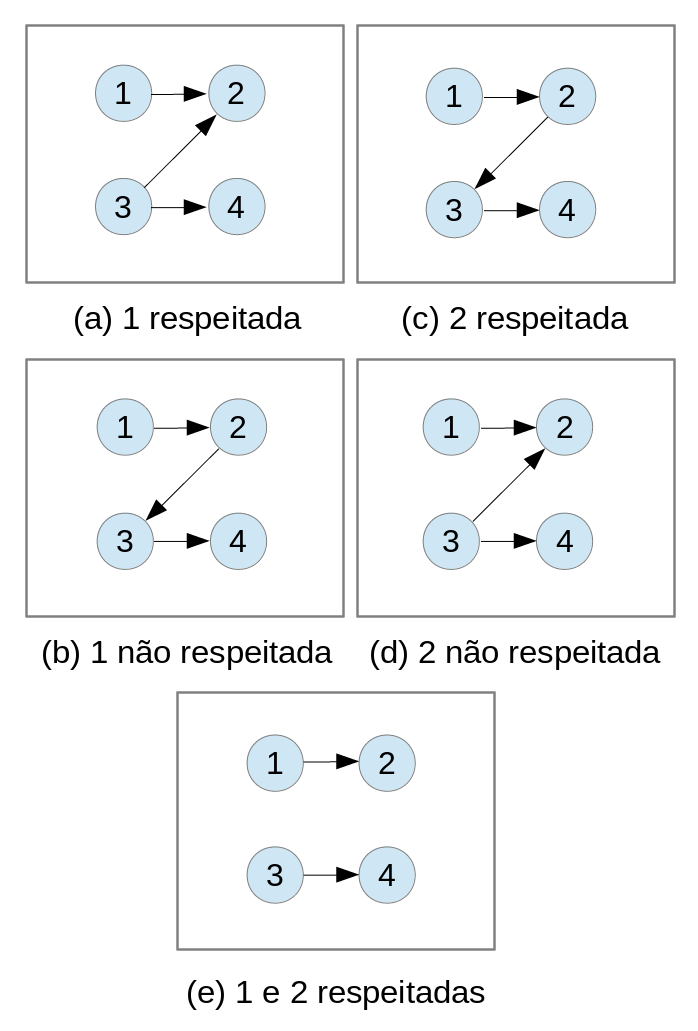
\includegraphics[width=0.7\textwidth]{figs/primario}
\caption[Cenários com diferentes variações das caraterísticas.]
{Cenários com diferentes variações das caraterísticas.}
\label{fig:primario}
\end{figure}

\subsection{Teste de Interferência Primária}

Seja $i$ um enlace de um conjunto $C \subset E$. O nó transmissor e o nó receptor de $i$ são, respectivamente, $s_{i}$ e $r_{i}$. $C$ passa no Teste de Interferência Primária (TIP)\abbrev{TIP}{Teste de Interferência Primária} se, e somente se, $\forall i,j \in C, s_{i} \neq s_{j} \& s_{i} \neq r_{j} \& r_{i} \neq s_{j} \& r_{i} \neq r_{j}$. 

\subsubsection{Descrição do Algoritmo}

\begin{algorithm}[h]
	\SetVline
	{\bf input:} Conjunto de enlaces $C$\\
	\ForEach { $i \in C$}{
		\ForEach { $j \in C$, $j \neq i$}{
			\If { (( $s_{i}==s_{j}$ ) $||$ ( $s_{i}==r_{j}$ ) $||$ ( $r_{i}==s_{j}$ ) $||$ ( $r_{i}==r_{j}$ ))}{
				\Return FALSE
			}
		}
	}
	\Return TRUE
\caption{Algoritmo TIP}
\label{alg:tip}
\end{algorithm}

\subsubsection{Prova de Corretude}

O TIP apenas formaliza o que foi definido na subseção anterior. Portanto, o algoritmo está correto. 

\subsubsection{Análise da Complexidade}

Para o pior caso, $|C|=m$, então a complexidade de tempo é $O(m^2)$. A complexidade de espaço é definida pelo maior tamanho de $C$ possível, portanto, $O(m)$.

\subsection{Modelo de Interferência Secundária}

Como mencionado no capítulo \ref{cap:introducao}, o meio de transmissão é compartilhado, então o nó transmissor em um enlace pode interferir nos nós receptores de outros enlaces. Contudo, existe um limite de interferência aceitável que é baseado na SINR ({\it Signal to Interference plus Noise Ratio}) \abbrev{SINR}{Signal to Interference plus Noise Ratio}  dos nós receptores.

A Potência de Recepção $RP(s,r)$ de uma transmissão entre s e r é a potência com que um sinal transmitido por um nó transmissor $s$ a uma potência de transmissão $TP$ é recebido em um nó $r$ seguindo o modelo de propagação. Matematicamente,

\begin{equation}
RP(s,r) = \frac{TP}{(\frac{d_{sr}}{d_{0}})^{\alpha}}
\label{eq:rp}
\end{equation}

onde $\alpha$ é o coeficiente e $d_{0}$ é a distância de referência do modelo de propagação.

Com isso, dado um nó receptor $r_{i}$, consegue-se calcular a potência de recepção em $r_{i}$ em duas situações distintas:

\begin{itemize} %verificar se pode ter lista com 2 itens

\item quando o sinal é transmitido por $s_{i}$, ou seja, é a potência de recepção dentro do próprio enlace $i$; 
\item quando o sinal é transmitido por $s_{j}$, tal que $j \neq i$, ou seja, é a potência de recepção de um sinal transmitido em um outro enlace $j$. Nesse caso, a potência de recepção de tais sinais é chamada de interferência. 

\end{itemize}

Denomina-se Interferência Total $I(i,C)$ a soma das interferências que os nós transmissores de todos os outros enlaces de $C$ exercem sobre o nó receptor do enlace $i$. Ou seja,

\begin{equation}
I(i,C) = \sum_{j \neq i} RP(s_{j},r_{i})
\end{equation}

Finalmente, a $SINR(i,C)$ é a razão entre a potência de recepção em $r_{i}$ referente a transmissão no enlace $i$ e a interferência causada pelo ruído do ambiente $\gamma$ e a interferência total dos outros enlaces no conjunto $C$.

\begin{equation}
SINR(i,C) = \frac{RP(s_{i},r_{i})} {\gamma + I(i,C)}
\label{eq:sinr}  
\end{equation}

Dado um conjunto de enlaces $C$ e tendo calculado $SINR(i,C)$, $\forall i \in C$, compara-se os valores encontrados com uma constante $\beta$, que representa um valor numérico para o limite de interferência tolerado. Se a interferência for muito alta, o valor do denominador na Equação~\ref{eq:sinr} irá aumentar, fazendo o valor da $SINR(i,C)$ diminuir. 

\subsection{Teste de Interferência Secundária}

No modelo de interferência secundária, $\beta$ é um limite inferior, tal que, se $SINR(i,C) \geq \beta$ , $\forall i \in C$, então $C$ passa no Teste de Interferência Secundária (TIS)\abbrev{TIS}{Teste de Interferência Secundária}.

\subsubsection{Descrição do Algoritmo}

\begin{algorithm}[h]
	\SetVline
	{\bf input:} Conjunto de enlaces $C$\\
	\ForEach { $i \in C$}{
		\If {(( $SINR(i,C)<\beta$ ))}{
			\Return FALSE
		}
	}
	\Return TRUE
\caption{Algoritmo TIS}
\label{alg:tis}
\end{algorithm}

\subsubsection{Prova de Corretude}

O TIS apenas formaliza o que foi definido na subseção 2.2.2. Portanto, está correto.

\subsubsection{Análise da Complexidade}

Como itera-se sobre todos os enlaces de C para calcular $SINR(i,C)$, sua complexidade é $O(m)$. Devido o laço definido na linha 2 iterar sobre no máximo m enlaces, então a complexidade de tempo é $O(m^2)$. Analogamente ao TIP, a complexidade de espaço é $O(m)$.

\subsection{Viabilidade de Conjuntos}

Dados os modelos de interferência apresentados, se um conjunto de enlace $C$ passar em ambos os testes, então diz-se que $C$ é viável. O algoritmo para testar a viabilidade de um conjunto de enlaces é simplesmente a junção dos algoritmos anteriores.

\subsubsection{Descrição do Algoritmo}

\begin{algorithm}[h]
	\SetVline
	{\bf input:} Conjunto de enlaces $C$\\
		\If { (TIP(C)) $\&\&$ (TIS(C))}{
			\Return TRUE
		}
		\Else {
			\Return FALSE
		}
\caption{Algoritmo VIAVEL}
\label{alg:viavel}
\end{algorithm}

\subsubsection{Prova de Corretude}

A condicional da linha 2 garante que ambos os testes são executados e, somente ao passar necessariamente nos dois, um conjunto C é classificado como viável. Portanto, o algoritmo está correto.

\subsubsection{Análise da Complexidade}

O pior caso para o teste de viabilidade é quando o conjunto é viável, ou seja, todas as iterações do TIP e do TIS ocorrem. Para o maior tamanho de C possível, temos que a complexidade de tempo desse algoritmo é $O(m)+O(m^2)=O(m^2)$.

\subsection{Inviabilidade Hereditária}

Dados os modelos de interferência apresentados, se um conjunto de enlace $C$ passar em ambos os testes, então diz-se que $C$ é viável. Entretanto, nesta subseção, será analisado o que acontece quando C não é viável.

Em um primeiro cenário, assume-se que $C$ não passou no TIP. Nesse caso, pelo menos um nó de $C$ está participando de mais de um enlace, o que é proibido. Seja um conjunto $C'$, tal que $C' = C \cup \{i\}$, onde $i \in E$. A adição do novo enlace $i$ em $C$ pode: ({\bf i}) conectar dois nós contidos em $C$; ({\bf ii}) conectar um nó existente em $C$ a um novo nó; e ({\bf iii}) incluir dois novos nós conectados por $i$. 
  
Nas três situações descritas anteriormente, a adição do novo enlace $i$ para formar $C'$ não muda o fato de que $C$ não é viável, independentemente do efeito que $i$ cause no conjunto original $C$. Consequentemente, é possível notar que $C'$ também não é viável.

Em um segundo cenário, assume-se que $C$ passou no TIP, mas não passou no TIS. Nesse caso, $SINR(i,C) < \beta$, para algum enlace $i$. Seja um conjunto $C'$, tal que, $C' = C \cup \{j\}$, onde $j \in E$ e $C'$ também passa no TIP. A adição de um novo enlace ao conjunto $C$ para formar $C'$, apenas fará aumentar a interferência nos enlaces já contidos em $C$. Mesmo que a contribuição na interferência total seja pequena, podendo até ser desprezada, a adição de um novo enlace não muda o fato de que $C$ não é viável. Consequentemente, é possível notar que $C'$ também não é viável.

Os dois cenários apresentados garantem a seguinte propriedade: se um conjunto $C$ não é viável, independentemente de qual teste de interferência ele falhou, então qualquer conjunto $C'$, tal que $C \subset C'$ também não é viável. Usando o modelo de árvore de combinações apresentado na seção anterior, se uma combinação $C$ da árvore de combinações não é viável, então todos os seus descendentes na árvore também não são viáveis. Por isso, essa propriedade é denominada Inviabilidade Hereditária. 

Devido a Inviabilidade Hereditária, no processo de busca e verificação de viabilidade de todas as combinações de enlaces de uma rede, sabe-se que, ao encontrar qualquer combinação não viável, não é necessário testar a viabilidade de nenhum de seus descendentes. O ato de não testar os descendentes de uma combinação não viável pode ser chamado de ``podar'' a árvore. 

\section{Exemplo com Busca em Profundidade}

A rede modelada na Figura \ref{fig:grafo} será utilizada para construir esse exemplo. O objetivo é encontrar os conjuntos de enlaces viáveis dessa rede. 

Nesse exemplo, os nós foram distribuídos aleatoriamente em uma área quadrada de lado $2000m$. As potências de transmissão foram fixadas em $TP=350mW=24.7712dBm$ para todos os nós. Nesse cenário, $m=4$ enlaces foram definidos, $E(G)=\{A, B, C, D\}$. Uma descrição dos enlaces contendo a distância entre os nós e a potência de recepção pode ser encontrada na Tabela \ref{table:enlaces}. Os valores do coeficiente e da distância de referência do modelo de propagação utilizados foram, respectivamente, $\alpha=4,0$ e $d_0=1,0$m.

\begin{table}[h]
\centering
\caption[Descrição dos Enlaces.]
{Descrição dos Enlaces.}
\label{table:enlaces}
\begin{tabular}{lccc}
\hline
Enlace & Distância ($m$) & Potência de Recepção ($10^{-8}mW$)\\ \hline
A=(4,3)	& $322,583$	& $2,77047$\\
B=(2,1)	& $292,245$	& $4,11274$\\
C=(2,3)	& $192,006$	& $22,0730$\\
D=(5,6)	& $179,399$	& $28,9628$
\end{tabular}
\end{table}

Existem $2^4 = 16$ combinações de enlaces que são representados na árvore de combinações da \ref{fig:bp}. Uma Busca em Profundidade será executada para percorrer os vértices da árvore que serão verificados usando o algoritmo VIÁVEL. A ordem em que os vértices são visitados é $\{\{\}, \{A\}, \{A,B\}, \{A,B,C\}, \{A,B,C,D\}, \{A,B,D\}, \{A,C\}, \{A,C,D\}, \{A,D\},$ $\{B\}, \{B,C\}, \{B,C,D\},$ $\{B,D\}, \{C\}, \{C,D\}, \{D\}\}$ e pode ser verificada também na Figura \ref{fig:bp}. A Tabela \ref{table:resultadoviabilidade} mostra o resultado dos testes para cada combinação. 

\begin{figure}[htb]
\centering
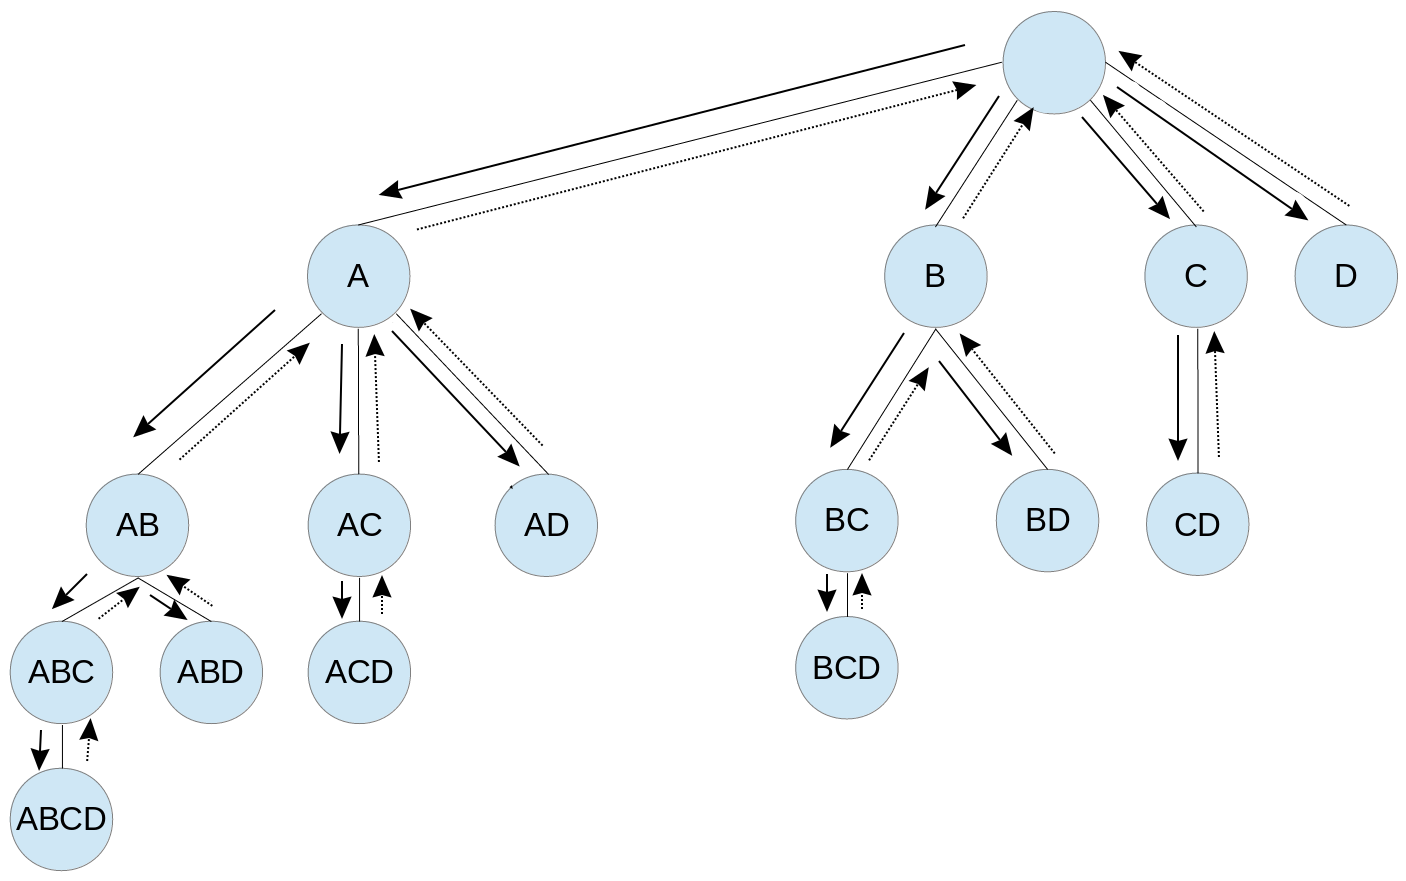
\includegraphics[width=1\textwidth]{figs/bp}
\caption[Busca em Largura na árvore de combinações.]
{Busca em Largura na árvore de combinações.}
\label{fig:bp}
\end{figure}

\begin{table}[h]
\centering
\caption[Resultados dos Testes de Viabilidade.]
{Resultados dos Testes de Viabilidade.}
\label{table:resultadoviabilidade}
\begin{tabular}{lcc}
\hline
Conjunto & Situação\\ \hline
\{\} & Dispensa teste\\
\{A\}	& Dispensa teste\\
\{A,B\}	& Falha TIS\\
\{A,B,C\}	& "Podado"\\
\{A,B,C,D\}	& "Podado"\\
\{A,B,D\}	& "Podado"\\
\{A,C\}	& Falha TIP\\
\{A,C,D\}	& "Podado"\\
\{A,D\}	& Falha TIS\\
\{B\}	& Dispensa teste\\
\{B,C\}	& Falha TIP\\
\{B,C,D\}	& "Podado"\\
\{B,D\}	& OK\\
\{C\}	& Dispensa teste\\
\{C,D\}	& OK\\
\{D\}	& Dispensa teste\\
\end{tabular}
\end{table}

O conjunto vazio e os conjuntos com apenas 1 enlace dispensam o teste de viabilidade. O primeiro conjunto a ser testado de verdade é o conjunto \{A,B\} que é reprovado no TIS e, portanto seus descendentes serão "podados". O conjunto \{A,C\} é reprovado no TIP pois A e C compartilham o nó 3 e, com isso, \{A,C,D\} é "podado". Em seguida, \{A,D\} é testado e reprovado no TIS, mas como é uma folha da árvore, a busca continua normalmente, sem "poda". O conjunto \{B,C\} é testado e reprovado no TIP pois B e C compartilham o nó 2 e, consequentemente, \{B,C,D\} é "podado". Finalmente, os conjuntos \{B,D\} e \{C,D\} são testados e classificados como viáveis, já que passam em ambos os testes.
Conclui-se que os conjuntos de enlaces viáveis obtidos são: $\{\{\},\{A\},\{B\},\{B,D\},\{C\},\{C,D\},\{D\}\}$. 

\begin{table}[H]
\centering
\caption{Cálculos das SINR}
\label{table:sinr}
\begin{tabular}{|c|l|c|c|c|}
\hline
\multicolumn{1}{|l|}{Combinação} & Enlaces($i=s_i,r_i$) & \multicolumn{1}{l|}{$d(s_j,r_i)${[}m{]}} & \multicolumn{1}{l|}{$I(j,i)[10^{-11}$mW$]$} & \multicolumn{1}{l|}{$SINR(i, \{i,j\}$){[}mW{]}} \\ \hline
                                 & C=(4,6)          & 1263,04                              & 11,7883                                  & \cellcolor[HTML]{9AFF99}1.115,22962           \\ \cline{2-5} 
\multirow{-2}{*}{\{C,D\}}        & D=(5,6)          & 1590,92                              & 4,68303                                  & \cellcolor[HTML]{9AFF99}2.282,86418           \\ \hline
                                 & B=(2,1)          & 1744,24                              & 3,24112                                  & \cellcolor[HTML]{9AFF99}365,73588             \\ \cline{2-5} 
\multirow{-2}{*}{\{B,D\}}        & D=(5,6)          & 1590,92                              & 4,68303                                  & \cellcolor[HTML]{9AFF99}2.282,86418           \\ \hline
                                 & A=(4,3)          & 1263,04                              & 11,78830                                 & \cellcolor[HTML]{FFCCC9}\textbf{139,97729}    \\ \cline{2-5} 
\multirow{-2}{*}{\{A,D\}}        & D=(5,6)          & 1327,55                              & 9,65865                                  & \cellcolor[HTML]{9AFF99}1.639,77421           \\ \hline
                                 & A=(4,3)          & 192,006                              & 22073,0                                  & \cellcolor[HTML]{FFCCC9}\textbf{0,12547}      \\ \cline{2-5} 
\multirow{-2}{*}{\{A,B\}}        & B=(2,1)          & 673,016                              & 146,224                                  & \cellcolor[HTML]{FFCCC9}\textbf{26,66666}     \\ \hline
\end{tabular}
\end{table}

A justificativa dos resultados dos TIS realizados são mostrados na Figura \ref{table:sinr}. O valor da tolerância de interferência escolhido foi $\beta=316,228$mW. A coluna das distâncias $d(s_j,r_i)$ mostra a distância entre transmissor de j ao receptor de i. Baseada nessa distância, a interferência total $I(j,i)$ na próxima coluna foi calculada. Na última coluna, o valor das {$SINR(i, \{i,j\}$  calculadas são listadas. Aquelas com valores menores que $\beta$ estão sombreadas de vermelho e justificam a combinação relacionada não ter passado no TIS. Para o cálculo da {$SINR(i, \{i,j\}$, o valor do ruído do ambiente utilizado foi $\gamma=8,004 \times 10^{-11}$ mW.

%No Apêndice A, é apresentada a justificativa para a escolha de todos os parâmetros para o Modelo de Interferência Secundária. Os parâmetros usados para construir esse exemplo também foram utilizados na parte de implementação para gerar as redes usadas nos experimentos. 

\section{Vantagens e Desvantagens}

No pior caso, o processo de enumeração descrito na seção anterior percorre todos os $2^m$ vértices da árvore, aplicando VIAVEL em cada conjunto de enlaces. Isso representa uma complexidade de $O(2^mm^2)$. Na prática, as redes possuem uma densidade grande. Por isso, é um exagero assumir que $2^m$ combinações serão testadas, pois certamente haverão muitos conjuntos não viáveis. 

Seja F o conjunto de combinações viáveis obtido por meio de um processo de enumeração como o da seção anterior. Certamente, $|F|$ combinações foram testadas, caso contrário não fariam parte de F. Na maioria dos casos, os conjuntos não viáveis são "podados" de forma que só um primeiro conjunto é testado. Supondo o pior caso, sempre depois de um conjunto viável com maior altura em um ramo da árvore ser testado, encontra-se um conjunto não viável. Nesse caso, o número de combinações testadas é igual a $|F| + |U|$, onde U é o conjunto das primeiras combinações não viáveis testadas depois de uma viável. É possível ver que $|F| \approx |U|$ e, portanto, o número de conjuntos testados é $2|F|$. 

Existe, então, um bom candidato a substituir a porção exponencial da complexidade do algoritmo mencionado. Como $O(|F|)$ conjuntos serão testados (viáveis ou não), a complexidade pode ser alterada para $O(|F|m^2)$. Até o momento, $|F|$ é desconhecido, mas certamente varia em função do tamanho da rede. No Capítulo \ref{cap:resultados}, uma função que represente os valores de $|F|$ usando m e n como parâmetros é aproximada, definindo melhor o valor da complexidade.

Mesmo com uma potencial redução da complexidade de tempo ao utilizar o valor $|F|$, a complexidade de espaço desse algoritmo ainda é exponencial. Isso significa que sua implementação está limitada a pequenos valores de m.

\section{Conclusão}

Nesse capítulo, todo o problema foi modelado usando diferentes abstrações com o intuito de obter um procedimento sistemático para enumerar combinações viáveis. Devido a essa modelagem, a complexidade de tempo encontrada em algoritmos que usam força bruta pode ser modificada para um valor diferente, que será estudado em capítulos futuros. Ainda assim, a complexidade de espaço continua exponencial, inviabilizando sua utilização na a maioria das aplicações.


  \chapter{Projeto do Algoritmo Iterativo}
\label{cap:iterativo}

\section{Introdução}

No Capítulo \ref{cap:modelagem}, uma abordagem foi utilizada para enumerar os conjuntos viáveis no exemplo proposto. Essa abordagem, possui elevada complexidade computacional e, por isso, não representa um bom candidato a ser implementado. Nesse capítulo, o algoritmo projetado será a primeira alternativa a essa abordagem.

O algoritmo introduzido aqui é composto por três partes básicas: codificação/decodificação, busca, e "poda". Ao reunir esses elementos, obtém-se um método iterativo para enumerar os conjuntos viáveis. Cada uma dessas partes será detalhada antes da descrição do algoritmo ser apresentada. Ao final, será feita uma análise de sua complexidade e comparação com o desempenho da abordagem anterior. 

\section{Representando Combinações Usando Inteiros}

\subsection{Codificação}

A primeira abstração a ser feita é considerar as combinações de enlaces como números binários. Nesses números, cada bit está relacionado à pertinência de um enlace específico àquela combinação. Consequentemente, também é possível representar a combinação de enlaces como um número inteiro sem sinal resultado da conversão do número na base 2 para a base 10. A seguir, essa modelagem é apresentada fazendo uso de uma linguagem mais formal, visando permitir algumas manipulações matemáticas importantes ao funcionamento do algoritmo.

Seja o grafo direcionado $G=(V,E)$. As m arestas em E são enumeradas como $e_0, e_1, e_2, ..., e_{m-1}$. Seja $B$ um número inteiro na base 2 com $m$ bits. Os bits em $B$ são enumerados como $b_0, b_1, b_2, ..., b_{m-1}$. Seja uma combinação de arestas $C$ tal que $C \in E$. O número $B$ codifica a combinação $C$ quando:

\[ b_i =
\begin{cases}
	1	\text{, sse } e_i \in C\\
	0	\text{, caso contrário}\\
  \end{cases}
\]

Essa ideia de codificação é estendida para toda a árvore de combinações. Ao fazer isso, todos os $2^m$ vértices da árvore serão codificados em inteiros.

% Figura 3.1: Exemplo de Árvore de Combinações codificada

Na Figura 3.1 é ilustrada uma árvore de combinações para uma rede com $E=\{a,b,c,d\}$, ou seja, $m=4$. Na imagem, todos os $2^4 = 16$ vértices possuem sua identificação principal na primeira linha, o valor codificado na base 2 na linha de baixo e o valor convertido para a base 10 entre parênteses na última linha.

\subsection{Decodificação}

Para conhecer os enlaces pertencentes a uma combinação e realizar o teste de viabilidade apropriadamente, é essencial que tal número possa ser decodificado em uma combinação de enlaces. A seguir, um algoritmo recursivo para decodificar um inteiro em um conjunto de enlaces é apresentado. Vale ressaltar que o processo de decodificação é o responsável por não ser preciso instanciar toda uma árvore de combinações. Com ele, é suficiente conhecer o conjunto de enlaces $E$ e os índices dos bits de $B$ para realizar os testes de interferência.

\subsubsection{Descrição do Algoritmo}

\begin{algorithm}[h]
	\SetVline
	{\bf input:} Número inteiro$B$, número inteiro $I$, conjunto de arestas $E(G)$\\
	$Q \leftarrow B/2$\\
	$R \leftarrow B\%2$\\
	\If{($R=1$)}{
		$C \leftarrow C \cup \{e_I\}$\\
	}
	\If{($Q>0$)}{
		$I \leftarrow I + 1$\\
		DECODIFICADOR(Q, I, E(G))\\
	}
\caption{Algoritmo DECODIFICADOR}
\label{alg:decodificador}
\end{algorithm}

\subsubsection{Prova de Corretude}

O algoritmo apresentado nada mais é do que uma versão recursiva do algoritmo padrão de conversão de um número na base 10 para a base 2 com uma modificação para permitir a captura dos enlaces pertencentes ao conjunto.

Nesse algoritmo existem duas variáveis de controle, $Q$ e $R$, que são, respectivamente, o quociente e o resto da divisão inteira entre os números $B$ e 2. Se $R=1$, temos $b_I=1$ e, consequentemente, o enlace $e_I$ pertence à combinação $C$ decodificada a partir do inteiro $B$. Reciprocamente, se $b_I=0$, então o enlace $e_I$ não pertence a $C$. A variável $Q$ controla a parada do algoritmo. Enquanto $Q>0$, o processo continua incrementando o valor de $I$ e verificando a pertinência dos enlaces com novos índices $I$. Quando $Q=0$, o processo de conversão é finalizado.

Quando $R=1$, então a condição na linha 3 é satisfeita e o enlace com índice $I$ é adicionado ao conjunto decodificado na linha 4. Portanto, ao final da recursão, $C$ será o conjunto de enlaces decodificado apropriadamente.

\subsubsection{Análise de Complexidade}

Todas as linhas do algoritmo são $O(1)$. Contudo, como trata-se de um algoritmo recursivo, a função Decodificador será chamada o número de vezes equivalente ao índice do bit ativo mais significativo. No pior caso, teremos $m-1$ chamadas da função, o que define sua complexidade de tempo como $O(m)$. Para o processo de decodificação é preciso armazenar, no máximo, $m-1$ enlaces e, portanto, sua complexidade de espaço é O(m).

\section{Percorrendo a Árvore Iterativamente}

No exemplo da Figura 3.1, foi visto que, para uma rede com $4$ enlaces, tem-se uma árvore de combinações com $16$ vértices. A árvore é estruturada da raiz ($C=\emptyset$ ou $B=0$) à sua folha de maior altura ($C=E$ ou $B=15$). De forma geral, para um grafo com $m$ enlaces, a árvore possui $2^m$ vértices, partindo de $B=0$ e chegando a $B=2^m-1$.

Na árvore codificada, a ordem em que os enlaces são considerados é muito importante porque os índices dos bits de $B$ são estritamente relacionados aos enlaces $e$, consequentemente, cada combinação $C$ é codificada unicamente por um número $B$.

Sabendo disso, é possível percorrer a árvore de combinações simplesmente realizando uma contagem que vai de 0 até $2^m -1$. Ou seja, todo vértice codificado $B>0$ é alcançado a partir da soma de um outro nó codificado mais $1$.

% Figura 3.2: Exemplo de como percorrer a Árvore de Combinações através da contagem

A Figura XXX mostra como a árvore do exemplo anterior é percorrida através da contagem. Comparado com o método de busca adotado no capítulo anterior, é importante ressaltar que a ordem em que os vértices são visitados é totalmente diferente. Essa nova ordem é consistente com uma contagem que somente é alcançável devido a codificação aqui introduzida.

\section{“Podando” a Árvore de Combinações}

Diferente do caso anterior, a vantagem em codificar as combinações para a atividade de ``poda'' da árvore não é tão trivial. Contudo, o método de busca baseado na contagem será usado para detectar alguns padrões que ajudam a “podar” a árvore de maneira eficiente. Mais uma vez, a correspondência entre $E$ e $B$ é muito importante e sua ordem, uma vez arbitrada, deve ser mantida no decorrer do processo. 

Dado um inteiro $B$, seus bits $b_i$ podem fornecer mais informações úteis além da pertinência do enlace $e_i$ ao conjunto $C$. Considere o caso em que $b_i^*$ é o bit ativo menos significativo, ou seja, é o bit 1 mais à direita. Nesse caso, o índice $i$ de $b_i^*$ também representa o número de filhos que $B$ tem na árvore, ou seja, quantas combinações são consequências diretas, ou descendentes diretos, de $C$. Em termos de bits, $i$ representa os números que são resultantes da variação dos bits 0 à direita de $b_i^*$ em $B$.

Isso significa que $b_i^*$ tem muito a dizer sobre os descendentes de $B$. Especificamente, se essa ideia for aplicada de maneira recursiva aos filhos $B'$ de $B$, seus $b_i^*$’s vão indicar o número de netos de $B$ e assim por diante. Ao final da recursão, uma combinação $C$ que foi codificada em $B$ tal que $b_i^*$ é o bit ativo menos significativo tem exatamente $2^i–1$ descendentes na árvore.

No capítulo 2, baseado na ideia de inviabilidade hereditária, o termo “podar” a árvore foi definido como o ato de ignorar os descendentes de uma combinação não viável ao percorrer uma árvore. Para o presente caso, como uma contagem está sendo feita, um termo mais adequado seria “saltar”. Portanto, uma vez que uma combinação codificada $B$ não for viável, um “salto” na contagem será realizado sobre todos os seus descendentes.

Como o número de descendentes de uma combinação B é facilmente determinável usando $b_i^*$, caso seja necessário realizar um “salto” na contagem devido a inviabilidade de $B$, basta incrementar a contagem com o número de descendentes mais $1$. Ou seja, se $B$ não é viável, a próxima combinação a ser testada será $B + 2^i$, onde $i$ é o índice do bit ativo menos significativo.

% Figura 3.3: Exemplo de contagem com “saltos”

Um exemplo de cenário em que os “saltos” ocorrem é ilustrado na Figura 3.3. Na rede do exemplo, sabe-se que as combinações $4$ e $12$ não são viáveis. Por isso, todos os descendentes de $4$ e de $12$ serão ignorados na contagem, resultando na sequência $0, 1, 2, 3, 4, 8, 9, 10, 11, 12$. Até esse ponto, as combinações de enlaces viáveis ainda não estão sendo listadas, apenas está sendo mostrada a sequência de enlaces visitados na contagem.

\section{Algoritmo Iterativo para Enumeração de Conjuntos de Enlaces Viáveis}

Finalmente, agora que os métodos de como percorrer a árvore de combinações, “saltar” sobre os descendentes das combinações inviáveis e decodificar os inteiros para realizar os testes de interferência são conhecidos, é possível descrever o algoritmo iterativo para enumeração de conjuntos de enlaces viáveis.

\subsubsection{Descrição do Algoritmo}

\begin{algorithm}[h]
	\SetVline
	{\bf input:} Grafo direcionado $G=(V,E)$\\
	{\bf output:} Conjuntos de Enlaces Viáveis $F$\\
	$F \leftarrow \emptyset$\\
	$C \leftarrow \emptyset$\\
	$B \leftarrow 0$\\
	$I \leftarrow 0$\\
	\While{$B<2^m$}{
		$C \leftarrow DECODIFICADOR(B, 0, E(G))$\\
		\If{$VIAVEL(C)$}{
			$F \leftarrow F \cup {B}$\\
			$I \leftarrow 1$\\
		}
		\Else{
			$I \leftarrow 2^i$\\
		}
		$B \leftarrow B + I$\\
	}
\caption{Algoritmo ITERATIVO}
\label{alg:iterativo}
\end{algorithm}

\subsubsection{Prova de Corretude}

De acordo com o que foi provado na seção XXX, o laço instanciado na linha 5 e o incremento feito na linha 12 representam uma contagem e, de fato, fazem o algoritmo percorrer todas as combinações de enlaces. Caso uma combinação seja viável, ela passará no teste da linha 7 e será adicionada ao resultado final na linha 8.

Os “saltos” demonstrados na seção XXX são baseados na variável $I$, usada como incremento à variável $B$. Pelo algoritmo, $I$ somente possui dois valores possíveis. 

\[ I =
\begin{cases}
	1	& \quad	\text{se, e somente se, } B \text{ é viável} \\
	2^i	& \quad	\text{caso contrário} \\
  \end{cases}
\]

Essa seleção de valores é gerenciada pela condicional das linhas 7 e 10.

Devido a inviabilidade hereditária, todos os $2^i$ descendentes de uma combinação inviável certamente também são inviáveis. Portanto, os “saltos” apenas tem o papel de agilizar o processo e não interferem no resultado final do algoritmo.

Conclui-se que, de fato, o algoritmo retorna todos os conjuntos de enlaces viáveis e, portanto, está correto.

\subsubsection{Análise de Complexidade}

O processo de decodificação apresentado é responsável por tornar desnecessário o armazenamento de todas as combinações de enlaces possíveis, como precisava ser feito na abordagem do capítulo anterior. Portanto, a complexidade de espaço é reduzida de $O(2^m)$ para $O(m)$.

	As linhas 1-4, 7-12 são $O(1)$. A função de decodificação na linha 6 é $O(m)$ e o teste de viabilidade na linha 7 é $O(m^2)$. O laço principal das linhas 5-12 é $O(2^mm^2)$ pois a cada uma das $2^m$ iterações (no pior caso), a função de decodificação e o teste de viabilidade são chamados com complexidade de $O(m) + O(m^2) = O(m^2)$. De maneira geral, a complexidade de tempo total é  $O(2^mm^2)$. 

Analogamente ao que foi explicado no capítulo anterior, esse valor de complexidade é muito exagerado e também cabe fazer a substituição de $2^m$ por $|F|$. Portanto, a complexidade é $O(|F|m^2)$.

\section{Conclusão}

Nesse capítulo, uma ideia de como percorrer a árvore em busca de combinações viáveis foi formalizada na forma de um algoritmo iterativo. Diferente da abordagem do capítulo anterior, devido ao processo de decodificação, apenas o conjunto de enlaces precisa ser armazenado, reduzindo consideravelmente sua complexidade de espaço. Contudo, sua complexidade de tempo continua a mesma do caso anterior.

  \chapter{Algoritmo Recursivo}
\label{cap:recursivo}

\section{Introdução}

Neste capítulo, será introduzido um novo algoritmo para encontrar os conjuntos de enlaces viáveis em uma rede sem fio. Esse algoritmo é baseado nos mesmos modelos apresentados no Capítulo \ref{cap:modelagem}, portanto ele possui algumas similaridades como o Algoritmo Iterativo introduzido no Capítulo \ref{cap:iterativo}. 

Como será mostrado nas próximas seções, o diferencial consiste em uma nova maneira de percorrer a árvore, que permitirá que os cálculos da SINR dos enlaces em uma dada combinação sejam reutilizados por seus descendentes. Finalmente, o algoritmo será detalhado e sua complexidade analisada.

\section{Percorrendo a Árvore Recursivamente}

A grande diferença com relação ao Algoritmo Iterativo está na forma em que a árvore é percorrida. No caso iterativo, faz-se uma contagem, ou seja, visita-se os vértices da árvore somando 1 ao seu valor codificado anterior. O caso recursivo não é tão simples e essa seção será dedicada ao seu entendimento.

Como foi mencionado no capítulo anterior, é possível saber quantos descendentes tem um conjunto codificado $B$. Para isso, basta encontrar o bit ativo menos significativo $b_i^*$ (o bit 1 mais à direita) e o número de bits 0 depois de $b_i^*$ é o número de filhos de $B$. Como consequência disso, é possível notar que as folhas da árvore possuem os seus bits menos significativos ativos, ou seja, se $B$ é ímpar, então $B$ é folha. Um caso especial surge ao analisar $B=0$. Nesse caso, não existem bits ativos e, por convenção, o número de filhos de $B=0$ é $|B|$.

Além de saber quantos filhos tem a combinação $B$, conhecer $b_i^*$ também nos permite alcançar os filhos de $B$. Para adicionar mais um enlace em $C$ e, com isso, descobrir um possível filho de $B$ na árvore, basta que um dos bits 0 depois de $b_i^*$ seja alternado para 1. De maneira geral, para fazer essa alternância, basta realizar a soma $B + 2^i$, tal que, $i < i^*$. Consequentemente, para alcançar todos os filhos de uma combinação B basta fazer $B + 2^i$, $\forall i$, tal que, $0\leq i\leq i^*$. Portanto, uma pequena contagem é feita para alternar todos os bits 0 depois de $b_i^*$ em uma combinação $B$ com o intuito de encontrar os filhos de $B$.

De maneira análoga, os netos de $B$ podem ser encontrados por meio da aplicação da técnica descrita nos filhos de $B$. Em geral, para encontrar todos os descendentes de uma combinação $B$, basta aplicar recursivamente a técnica em cada descendente de $B$. Quando a recursão alcançar uma folha, essa instância se encerra. Se a técnica descrita for aplicada para $B=0$, então todos os seus descendentes serão alcançados e, portanto, toda a árvore de combinações será visitada. Um exemplo de como percorrer uma árvore com $m=4$ é apresentado na Figura 4.1.

% Figura 4.1: Percorrendo a Árvore Recursivamente

\section{“Podando” a Árvore de Combinações}

“Podar” uma árvore de combinações que esteja sendo percorrida usando o método da seção anterior é muito mais simples do que “saltar” em uma contagem. Quando uma folha $B' = B + 2^i$ na árvore é alcançada, como ela não tem filhos, a técnica não será mais aplicada e instância da busca que visitou tal folha é encerrada, de forma que a busca continua em $B''=B+2^i+1$. O mesmo acontece quando uma combinação $B'$ visitada não é viável. Nesse caso, todos os descendentes de $B'$ são ignorados e a busca continua em $B'$.

Dada essa situação, é importante ressaltar que, nem sempre irá existir um $B''$, ou seja, um vértice irmão de $B'$. Caso isso venha a acontecer, significa que todos os descendentes de um vértice já foram visitados (ou ignorados) e ele é o último em seu ramo com altura $h$, ou seja, o último filho de $B$. Isso fará com que sua instância da recursão se encerre e autoriza o seu pai na árvore a visitar algum outro filho, se houver. 

\section{Reaproveitando Cálculos}

No algoritmo anterior, era fundamental que houvesse um processo de decodificação do número $B$ em um conjunto $C$ para que os testes de interferência fossem realizados. No caso da busca recursiva, quando um novo vértice é visitado, o enlace $e_i$ correspondente ao índice $i$ do bit alternado é adicionado em $C$. Ao ser adicionado em $C$, a porção de interferência causada e sofrida por $e_i$ é atualizada. A viabilidade do conjunto $C$ é testada toda vez que um novo enlace é adicionado. Simetricamente, depois de visitar todos os seus descendentes, $e_i$ é removido de $C$.

Ao realizar o procedimento de adição e remoção dos enlaces descrito, dado um conjunto viável $B$, para testar a viabilidade de seus filhos na árvore, basta considerar a contribuição de interferência do enlace adicionado a $B$. Isso significa que todo o cálculo de SINR feito de 0 até $B$ não precisa ser refeito ao testar os filhos de $B$.

Além disso, a SINR já é calculada no momento em que um novo enlace é adicionado ao conjunto. Logo, para esse caso, a complexidade do algoritmo TIS é reduzida. Como as SINR já estão calculadas, basta iterar sobre os enlaces de $C$, fazendo a complexidade de tempo diminuir de $O(m^2)$ para $O(m)$. Como será detalhado no Capítulo \ref{cap:resultados}, o tempo do TIS também será reduzido para $O(m)$. Consequentemente, o algoritmo VIAVEL para o caso recursivo terá complexidade $O(m) + O(m) = O(m)$. 

\section{Descrição do Algoritmo}

Até o momento, uma nova ideia de como percorrer a árvore foi apresentada. Essa ideia permite que a árvore seja “podada” e dispensa a necessidade de decodificação, o que, intuitivamente, representa um ganho na complexidade de tempo em relação ao Algoritmo Iterativo. O Algoritmo Recursivo é apresentado a seguir.

\subsection{Algoritmo Recursivo para Enumeração de Conjuntos de Enlaces Viáveis}

\subsubsection{Descrição do Algoritmo}

\begin{algorithm}[h]
	\SetVline
	{\bf input:} Grafo direcionado $G=(V,E)$, Conjunto de Enlaces $C$, Inteiro $X$\\
	{\bf output:} Conjuntos de Enlaces Viáveis $F$\\
	\If{$X=0$}{
		\For{$i=0$ to $m-1$}{
			$RECURSIVO(G, C, X + 2^i)$\\
		}
	}
	\Else{
		$limite \leftarrow log2(X \& ~(X-1))$\\
		$C \leftarrow C \cup \{e_{limite}\}$\\
		\If{$VIAVEL(C)$}{
			$F \leftarrow F \cup {C}$\\
			\For{$i=0$ to $limite-1$}{
				$RECURSIVO(G, C, X + 2^i)$\\
			}
			$C \leftarrow C \ {e_{limite}}$\\
		}
	}
\caption{Algoritmo RECURSIVO}
\label{alg:recursivo}
\end{algorithm}

\subsubsection{Prova de Corretude}

Como mostrado na seção 4.2, se $X=0$, então toda a árvore é percorrida chamando o algoritmo RECURSIVO recursivamente para todos os descendentes. A condicional na linha 1 e 4 fazem o tratamento do caso especial em que $X=0$. A chamada recursiva da função só é feita quando o conjunto $C$ se mostra viável ou quando $limite>0$. Se $C$ não é viável então RECURSIVO não será chamada para seus descendentes, o que não problema devido a Inviabilidade Hereditária. Logo, ignorar os descendentes de uma combinação não viável não altera o resultado do algoritmo, apenas agiliza o processo. As linhas 6 e 11 garantem que qualquer enlace que seja adicionado a $C$ também seja removido. Finalmente, na linha 8, se $C$ é viável, então é adicionado ao conjunto $F$ e, por isso, $F$ contém todos os conjuntos de enlaces viáveis. Portanto, o algoritmo está correto.

\subsubsection{Análise da Complexidade}

Assim como no caso do algoritmo ITERATIVO, a complexidade de espaço é $O(m)$.

A complexidade de tempo desse algoritmo é parecida com a do algoritmo ITERATIVO. Contudo, como houveram algumas otimizações decorrentes do reaproveitamento dos cálculos da SINR, sua complexidade é um pouco menor. Houve uma redução de $O(|F|m^2)$ para $O(|F|m)$.

\section{Conclusão}

Apesar de uma concepção um pouco mais complexa, o algoritmo RECURSIVO obteve melhor complexidade de tempo em comparação com todas as técnicas apresentadas até agora. Tudo isso, devido a reutilização dos cálculos proporcionada por sua natureza recursiva. 

  \chapter{Implementação e Resultados}
\label{cap:resultados}

\section{Introdução}

Nos capítulos anteriores, os algoritmos ITERATIVO e RECURSIVO foram introduzidos trazendo menores complexidades do que a força bruta pura. Neste capítulo, será estudado o que tais complexidades representam em termos de recursos computacionais reais, ou seja, quanto de espaço em memória e tempo de processamento eles precisam. 

Além disso, detalhes de implementação relevantes como teconologias e ambientes adotados são descritos. Finalmente, todo o plano de simulações será detalhado e os resultados são analisados.

\section{Otimizações}

Antes de falar da implementação, é importante mostrar algumas ideias que ajudaram a reduzir ainda mais a complexidade dos algoritmos.

\subsection{Acoplamentos em Grafos}

Em Teoria dos Grafos, um acoplamento $M$ de um grafo $G=(V,E)$ é definido como um subconjunto de $E(G)$, tal que, para qualquer par de arestas $(i,j) \in M$, $i$ e $j$ não são adjacentes, ou seja, não compartilham vértices. Um acoplamento máximo $M^*$ é aquele com o maior número possível de arestas. 

A partir dessas definições, é possível extrair duas propriedades fundamentais:
\begin{enumerate}
\item Para qualquer $M$ em $G=(V,E)$, $g(v) \leq 1, \forall v \in V(G)$
\item Para qualquer $M^*$ em $G=(V,E)$, $|M^*|= \lfloor n/2 \rfloor$
\end{enumerate}

\subsection{Limitando a Busca}

O Modelo de Interferência Primária, devido algumas características, não permite que nós da rede estejam participando de mais de um enlace de comunicação ao mesmo tempo. Logo, em uma rede modelada por um grafo $G=(V,E)$, um conjunto de arestas $C \subset E(G)$ é viável se, e somente se, as arestas de $C$ não comparilham vértices, ou seja, não são adjacentes entre si. 

Dada a definição na seção anterior, um conjunto viável $C$ é um acoplamento $M$ de $G$. Portanto, o maior tamanho possível para um conjunto viável $C^*$ é o tamanho de um acoplamento máximo $M^*$, ou seja, $|C^*| = |M^*| = \lfloor n/2 \rfloor$. Com essa informação, é possível "podar" todos os vértices $C$ da árvore de combinações que tenham $|C|>n/2$, conforme exemplificado na Figura 5.1.

%Figura
\begin{figure}[ht] 
  \label{fig:otimizacao} 
  \begin{minipage}[b]{0.5\linewidth}
    \centering
    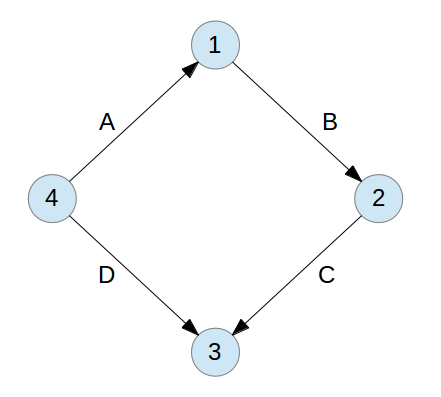
\includegraphics[width=0.5\linewidth]{figs/otim1.png} 
    \caption{Grafo com $n=m=4$} 
    \vspace{4ex}
  \end{minipage}%%
  \begin{minipage}[b]{0.5\linewidth}
    \centering
    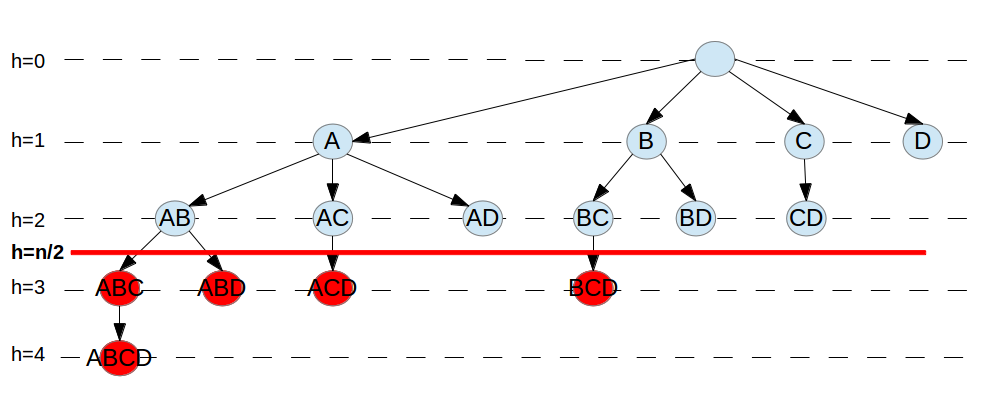
\includegraphics[width=1\linewidth]{figs/otim2.png} 
    \caption{Árvore "podada em $n/2$} 
    \vspace{4ex}
  \end{minipage} 
\end{figure}

Usando essa técnica, a complexidade para percorrer a árvore cai de $O(2^m)$ para $(2^{n/2})$.

\subsection{Reformulando o TIP}

Como consequência da definição de acoplamento, é possível reescrever o algoritmo \ref{alg:tip} com uma menor complexidade.

\subsubsection{Descrição do Algoritmo}

\begin{algorithm}[h]
	\SetVline
	{\bf input:} Conjunto de enlaces $C$\\
	\ForEach { $i \in C$}{
			\If {(($g(s_{i})>1$)$||$($g(s_{i})>1$))}{
				\Return FALSE
			}
	}
	\Return TRUE
\caption{Algoritmo TIP-G}
\label{alg:tipg}
\end{algorithm}

\subsubsection{Prova de Corretude}

Pela propriedade 1, se, dado um conjunto $C \in E(G)$, $\forall v \in V(G), g(V) \leq 1$, então C é um acoplamento e, portanto, C é viável. Isso garante que as arestas de C não compartilham vértices, ou seja, os nós do conjunto apenas participam de um enlace. Então, para testar a Interferência Primária, não é necessário verificar se em cada par de enlaces existem nós compartilhados. Basta verificar que o grau dos vértices nos enlaces de C são menores que 2. Como essa verificação é feita na linha 3, o algoritmo está correto.

\subsubsection{Análise de Complexidade}

A complexidade de espaço é O(m). Devido a otimização anterior, $m \leq n/2$, então a complexidade é reduzida a $O(n/2)=O(n)$. 

Como todos os enlaces de C são avaliados, então a complexidade é O(m). Contudo, sabemos que $|C| \leq n/2$, portanto, a complexidade de espaço é reduzida para $O(n)$

\section{Detalhes de Implementação}

Todos os algoritmos aqui apresentados, bem como as estruturas de dados subjacentes, foram implementados usando a liguagem de programação C++ sob o paradigma de Orientação a Objetos. O ambiente de desenvolvimento foi composto do sistema operacional Ubuntu 16.04 64 bits com o compilador GCC 5.4.0-6, usando o editor Atom para produção do código. O hardware utilizado foi um processador Intel Core i5-3337U com 6GB de RAM.

A primeira porção de código produzido foi referente a modelagem da rede. As classes Node, Link e Network representam os nós, enlaces e a rede, respectivamente. Além dos dados relevantes aos cálculos efetuados, como posição dos nós, potência de recepção, entre outros, vários métodos também foram criados, como geração aleaória da posição dos nós, cálculo da distância entre nós e assim por diante. O objeto da classe Network é servir de entrada para os algoritmos. 

Para geração das redes, três parâmetros são utilizados: (i) potência de transmissão TP; (ii) número de nós N; (iii) tamanho do lado A da área quadrada onde os nós serão dispostos. A primeira coisa a ser feita é distribuir os N nós aleatoriamente dentro da área definida por A. A distância entre todos os pares de nós é então calculada. Se a distância entre os nós for menor que um limite D, então um enlace é criado para conectá-los usando a equação \ref{eq:rp}.  

Devido algumas facilidades para gerenciar variáveis compartilhadas, os algoritmos ITERATIVO e RECURSIVO também foram codificados como classes, Iterative e Recursive, respectivamente. Ambas as classes possuem o método construtor e o método principal que implementa o algoritmo propriamente dito, além de alguns outros métodos secundários para manipulação dos dados.

A arquitetura do ambiente descrito é o principal limitante dos algoritmos. Como os processadores são de 64 bits, o maior número inteiro nativo oferecido pela linguagem C++ é $2^{64}-1$. Portanto, até o momento, não é possível aplicar esses algoritmos a redes com mais de 64 enlaces. Devido a essa limitação, alguns cuidados também tiveram que ter sido tomados. Por exemplo, em C++, em uma contagem, ao exceder o número $2^{64}-1$, a contagem é retomada do 0. Se nenhum mecanismo para detectar essa situação fosse implantado, ao executar os algoritmos para $m=64$, o programa iria entrar em loop infinito. Um outro caso é baseado na inicialização da variável $limite$. No algoritmo ITERATIVO, $limite = 2^m$, logo, se $m=64$, então $limite=0$ e, portanto, o programa seria encerrado antes mesmo de entrar no loop principal. Mais uma vez, um mecanismo teve de ser adotado para contornar essa situação.

\section{Simulações e Resultados}

\subsubsection{Verificação da variação da quantidade de conjuntos de enlaces viáveis}

É importante verificar a variação da quantidade de conjuntos de enlaces viáveis resultantes da execução dos algoritmos em função do tamanho da rede para melhor determinar a sua complexidade computacional. Para isso, 30 redes diferentes para cada valor de m e n foram geradas. Mais uma vez, $n=\{16,32,64,128\}$. 

Em cada uma dessas redes, o número de conjuntos viáveis foi computado. A média dos valores encontrados foi utilizada para gerar uma curva e, com isso, poder aproximar a complexidade dos algoritmos.

%Figura: Número médio de conjuntos viáveis
\begin{figure}[ht] 
  \label{fig:tamanho} 
  \begin{minipage}[b]{0.5\linewidth}
    \centering
    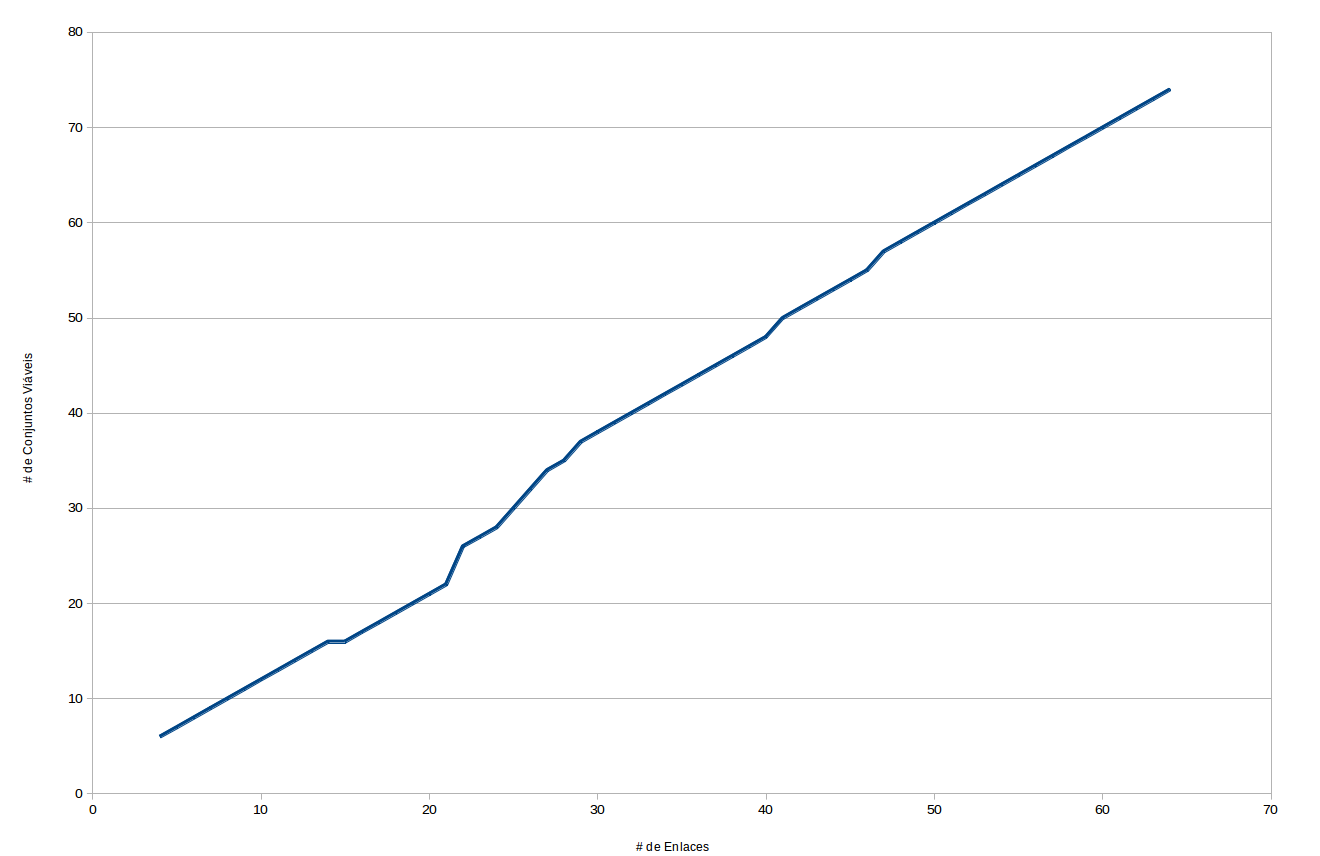
\includegraphics[width=1\linewidth]{figs/tamanho16.png} 
    \caption{Variação de $|F|$ para $n=16$} 
    \vspace{4ex}
  \end{minipage}%%
  \begin{minipage}[b]{0.5\linewidth}
    \centering
    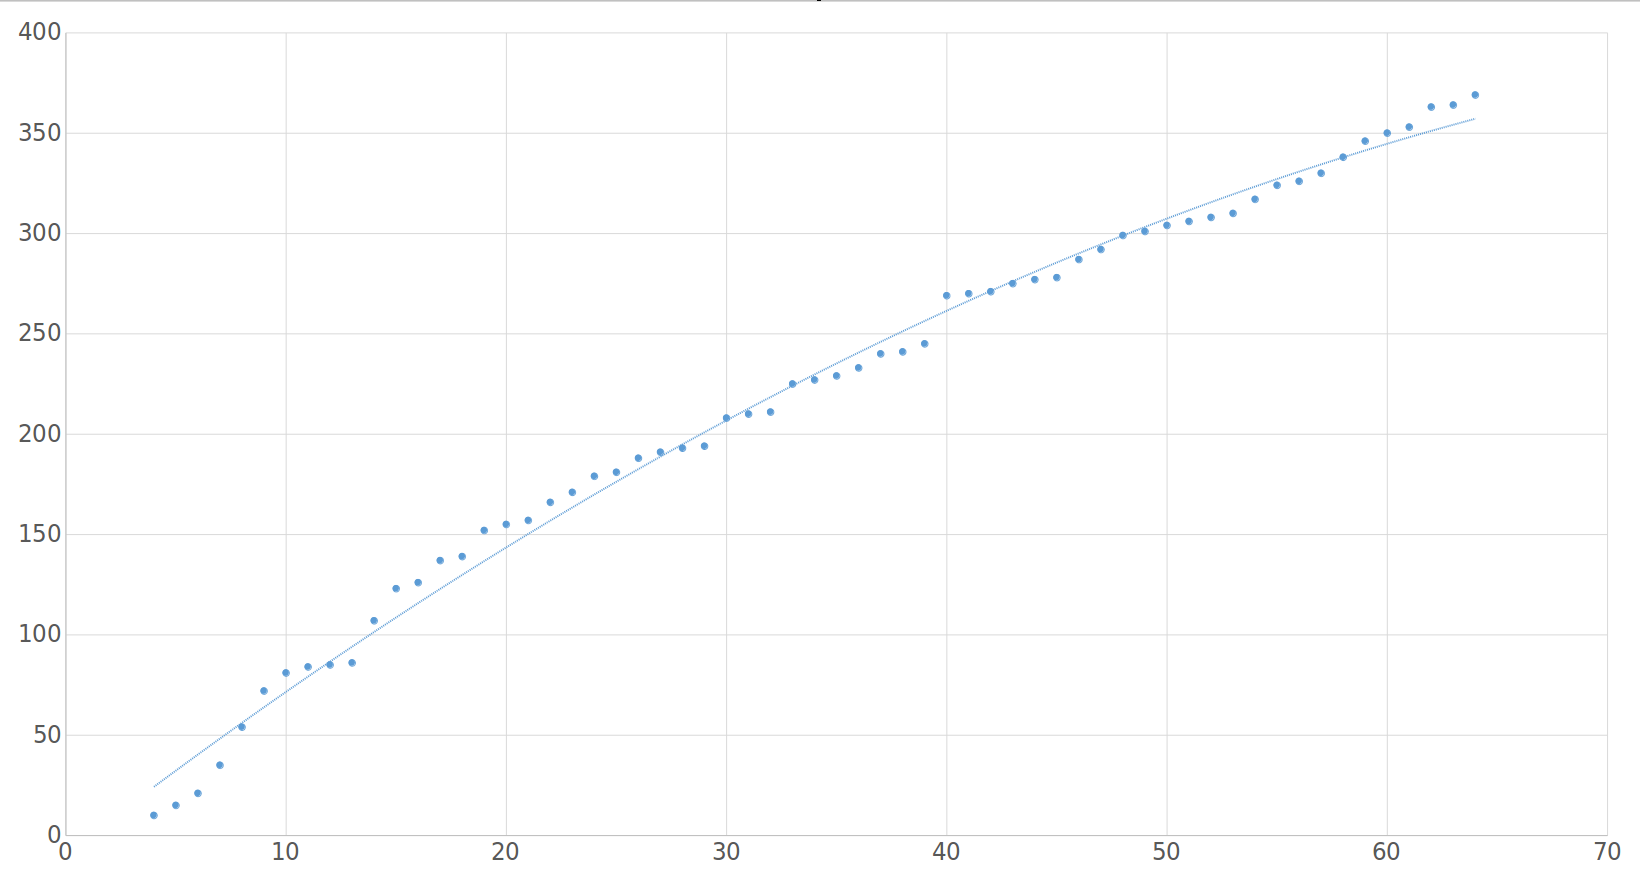
\includegraphics[width=1\linewidth]{figs/tamanho32.png} 
    \caption{Variação de $|F|$ para $n=32$} 
    \vspace{4ex}
  \end{minipage} 
  \begin{minipage}[b]{0.5\linewidth}
    \centering
    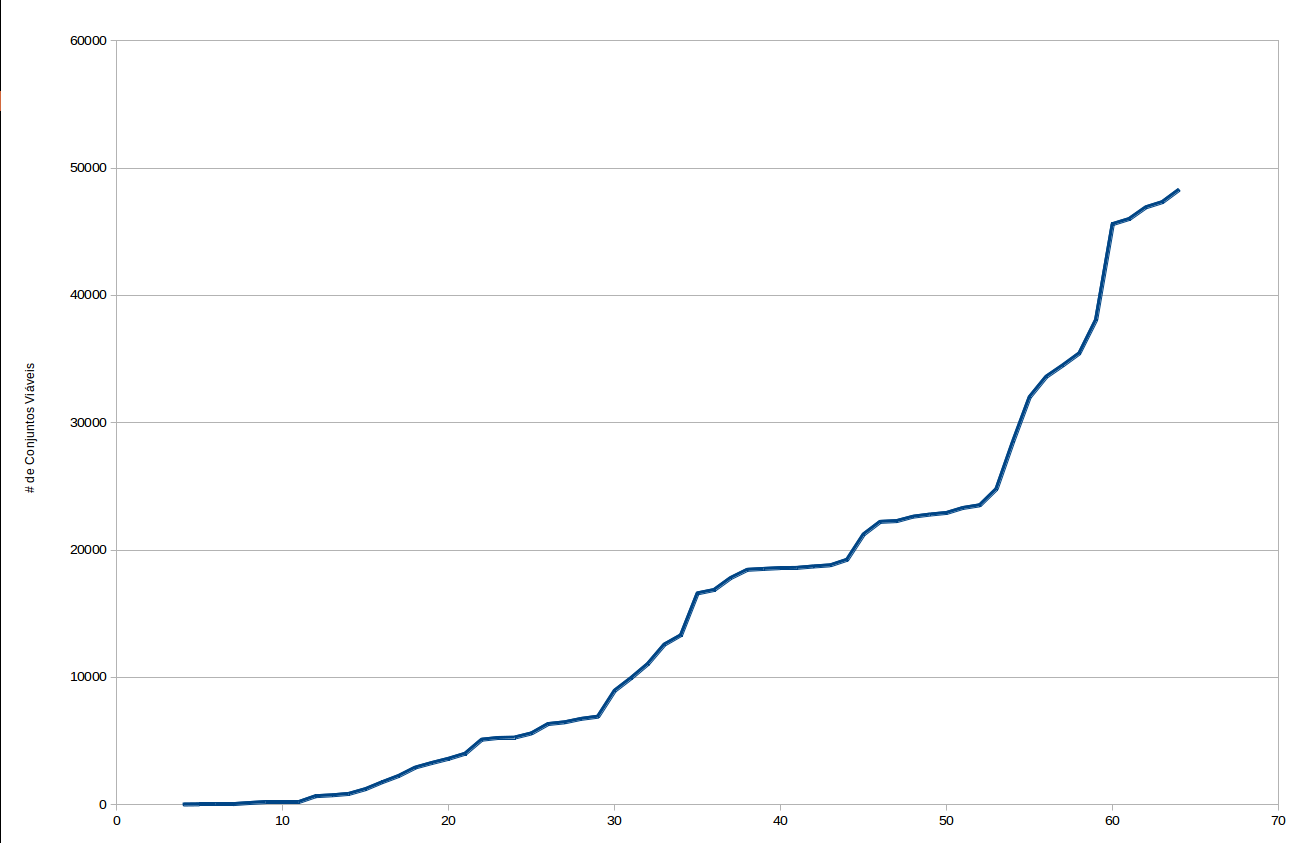
\includegraphics[width=1\linewidth]{figs/tamanho64.png} 
    \caption{Variação de $|F|$ para $n=64$} 
    \vspace{4ex}
  \end{minipage}%% 
  \begin{minipage}[b]{0.5\linewidth}
    \centering
    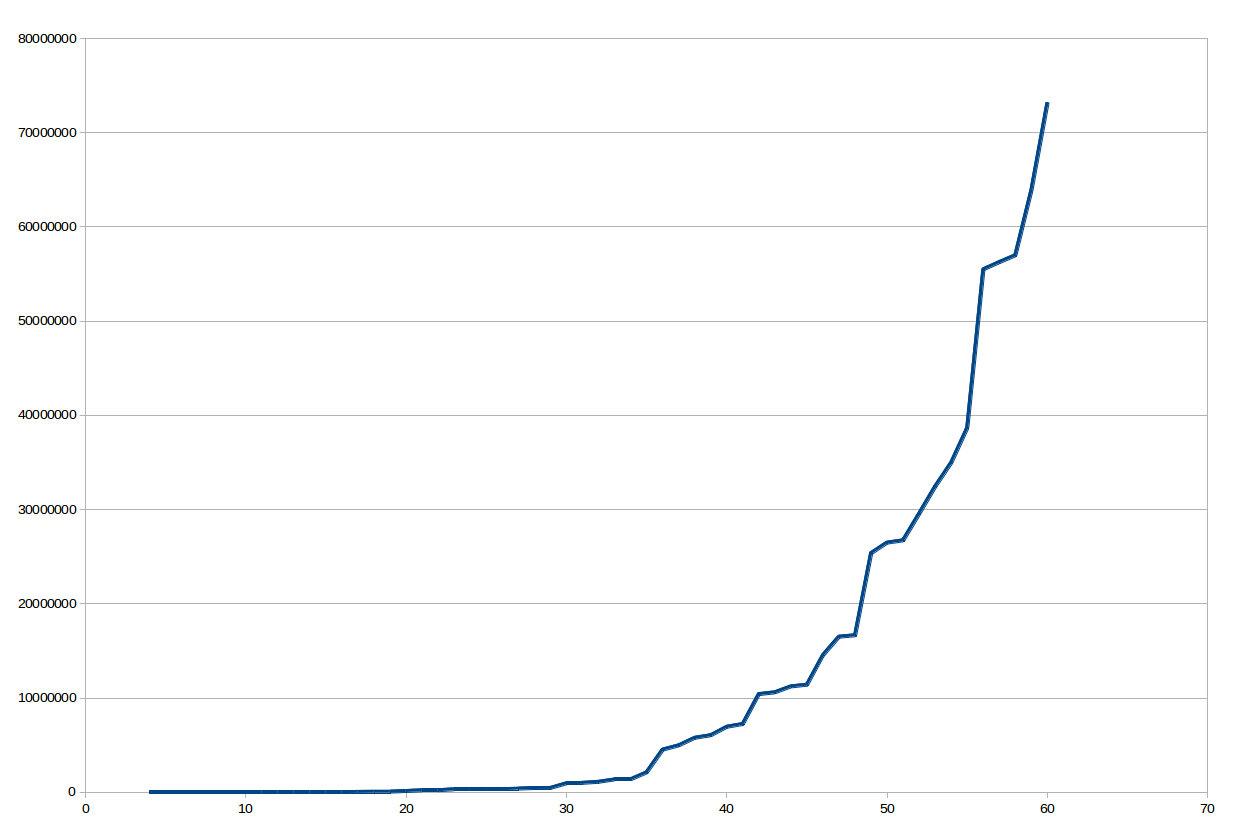
\includegraphics[width=1\linewidth]{figs/tamanho128.png} 
    \caption{Variação de $|F|$ para $n=128$} 
    \vspace{4ex}
  \end{minipage} 
\end{figure}

Assim como no caso anterior, as curvas se acentuam com o aumento de n. Isso significa que a variação do número de conjuntos viáveis torna-se mais sensível ao aumento do número de enlaces a medida que maiores valores de m são utilizados. 

O método de regressão linear foi utilizado para interpolar as curvas subjacentes aos gráficos da figura anterior. Usando esse método, foi possível encontrar uma função de f(m) que melhor se aproxima dos pontos, ou seja, que melhor descreve o comportamento do número de conjuntos em função de m. As funções encontradas para os diferentes valores de n são mostradas da tabela a seguir.

\begin{table}[h]
\centering
\caption[Funções Aproximadas]
{Funções Aproximadas.}
\label{table:funcoes}
\begin{tabular}{lc}
\hline
$n$ & $f_n(m)$\\ \hline
16  & $f_{16}(m) = am^2 + bm + c$\\
32  & $f_{32}(m) = am^2 + bm + c$\\
64  & $f_{64}(m) = am^2 + bm + c$\\
128 & $f_{128}(m) = am^2 + bm + c$\\
\end{tabular}
\end{table}

Em todos os casos, $f_n(m)$ é $O(n^2)$. Logo, é possível afirmar que $O(|F|)=O(n^2)$. Conclui-se que, as complexidades dos algoritmos ITERATIVO e RECURSIVO são, respectivamente, $O(|F|n^2) = O(n^2n^2) = O(n^4)$ e $O(|F|n) = O(n^2n) = O(n^3)$. Para o algoritmo RECURSIVO, a complexidade de tempo é menor do que a força bruta pura, que é $O(|F|n^2) = O(n^2n^2) = O(n^4)$. 

\subsubsection{Complexidades}

Agora que o valor de $O(|F|)$ foi encontrado, pode-se resumir as complexidades computacionais dos algoritmos apresentados nesse trabalho.

\begin{table}[h]
\centering
\caption[Complexidades Computacionais]
{Complexidades Computacionais.}
\label{table:complexidade}
\begin{tabular}{lcc}
\hline
Algoritmo & Tempo & Espaço\\ \hline
Força Bruta Pura & $O(2^mm^2)$ & $O(2^m)$\\
BP com "Poda" & $O(m^4)$ & $O(2^m)$\\
ITERATIVO & $O(m^4)$ & $O(m)$\\
RECURSIVO & $O(m^3)$ & $O(m)$\\
ITERATIVO + Otimizações & $O(n^4)$ & $O(m)$\\
RECURSIVO + Otimizações & $O(n^3)$ & $O(m)$\\
\end{tabular}
\end{table}

\subsubsection{Verificação do tempo de execução real dos algoritmos}

Para alcançar esse objetivo, um programa foi criado para variar o valor do lado da área A com o intuito de simular redes de 4 a 64 enlaces. Além do tempo de execução de cada algoritmo para as 60 redes geradas, também se mostrou importante entender o efeito da variação do número de nós. Os valores utilizados para n são $\{16, 32, 64, 128\}$. 

Então, as redes foram simuladas com diferentes valores de m e n e o tempo de execução de ambos os algoritmos foi medido. Para evitar ruídos provenientes de variações computacionais aleatórias, 30 execuções de cada algoritmo foram feitas para cada cenário, seguindo a regra de [Citar o cara que determinou esse número]. Ao final, o tempo médio das execuções foi utilizado para gerar uma curva e, com isso, poder analisar o tempo real.

\begin{figure}[ht] 
  \label{fig:tempo} 
  \begin{minipage}[b]{0.5\linewidth}
    \centering
    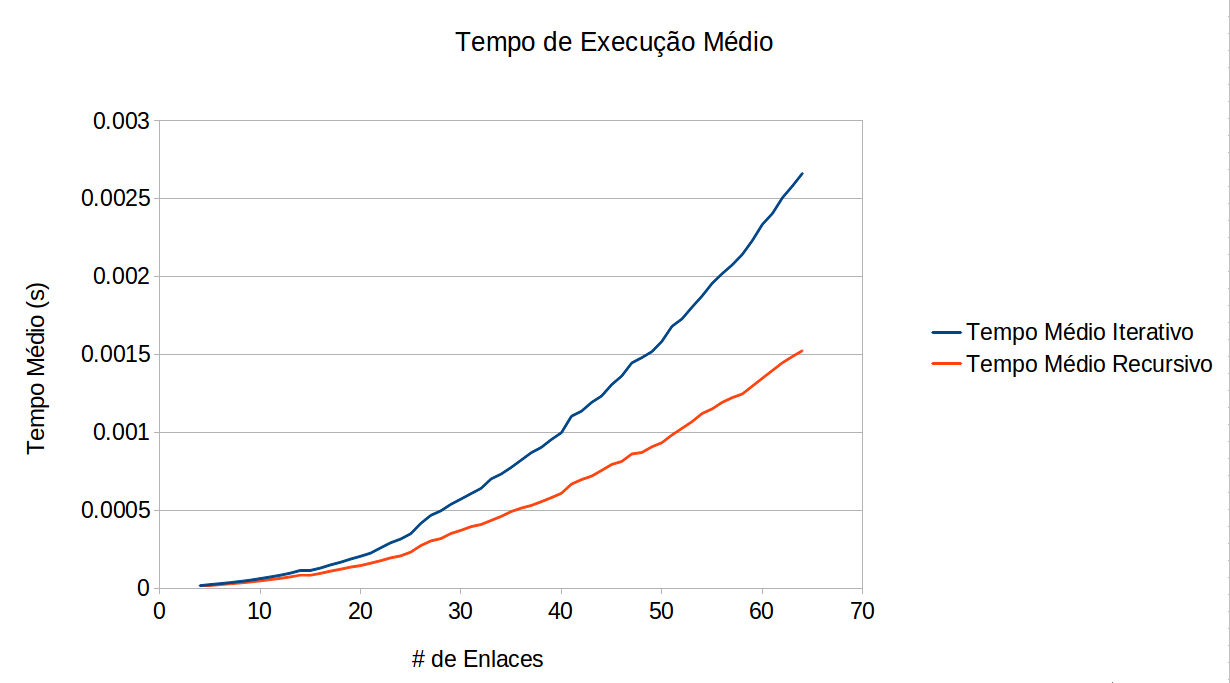
\includegraphics[width=1\linewidth]{figs/tempo16.png} 
    \caption{$n=16$} 
    \vspace{4ex}
  \end{minipage}%%
  \begin{minipage}[b]{0.5\linewidth}
    \centering
    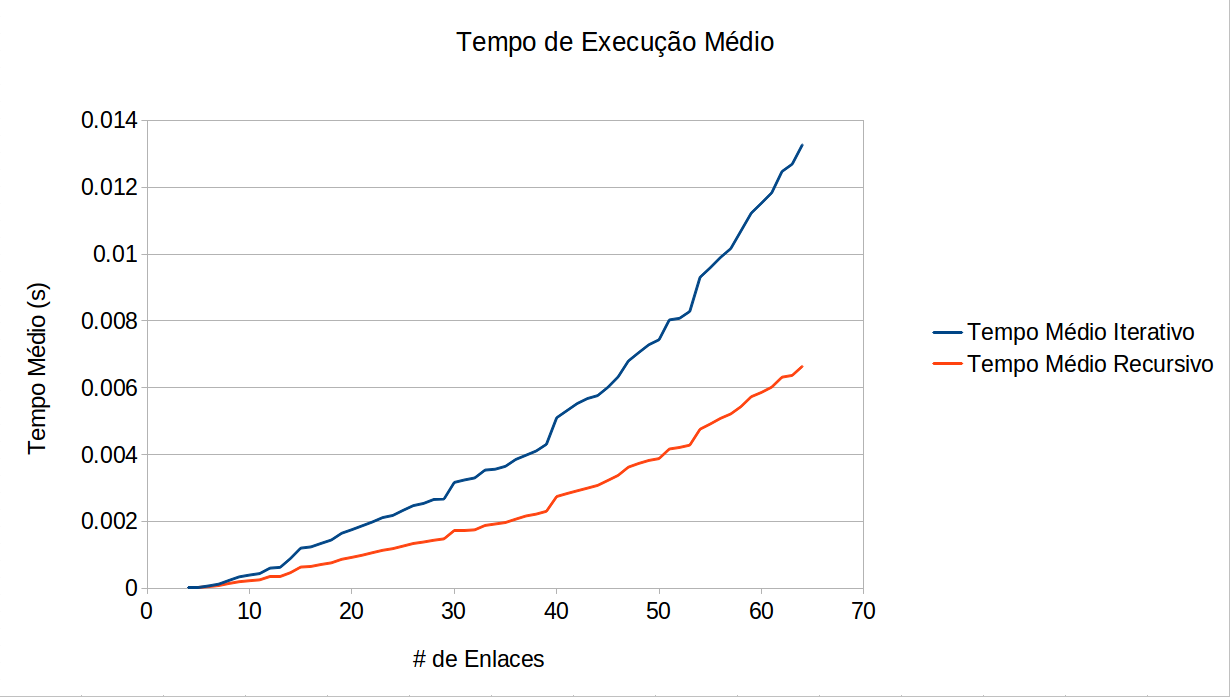
\includegraphics[width=1\linewidth]{figs/tempo32.png} 
    \caption{$n=32$} 
    \vspace{4ex}
  \end{minipage} 
  \begin{minipage}[b]{0.5\linewidth}
    \centering
    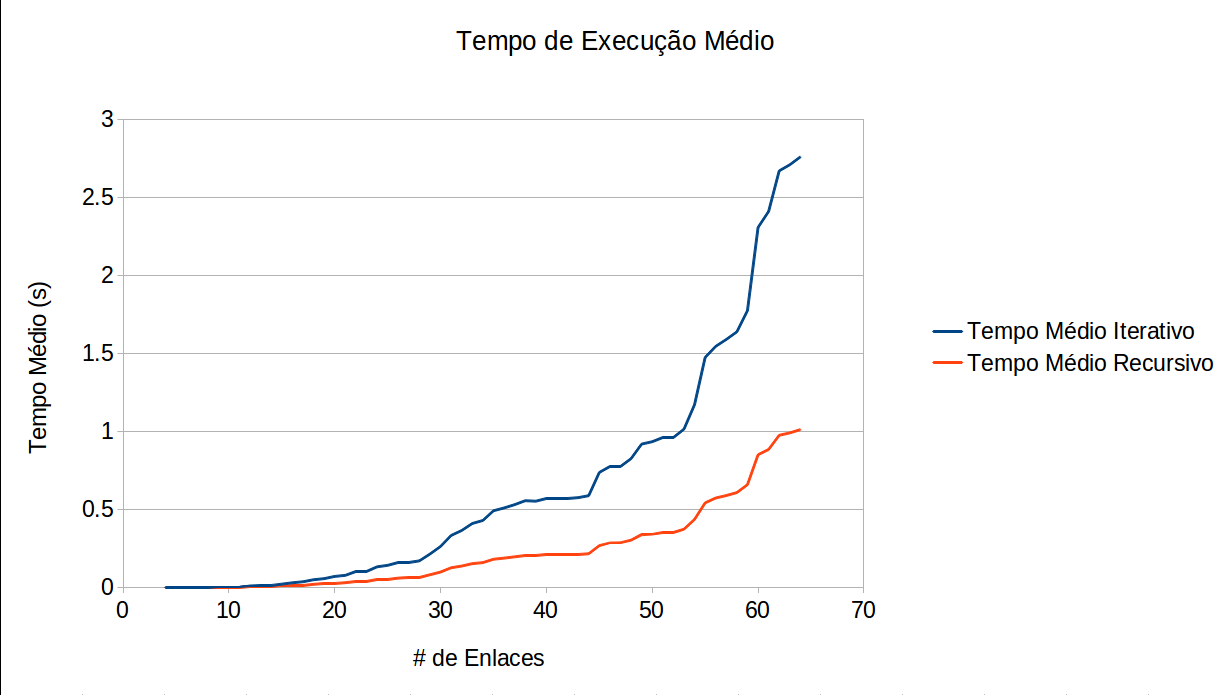
\includegraphics[width=1\linewidth]{figs/tempo64.png} 
    \caption{$n=64$} 
    \vspace{4ex}
  \end{minipage}%% 
  \begin{minipage}[b]{0.5\linewidth}
    \centering
    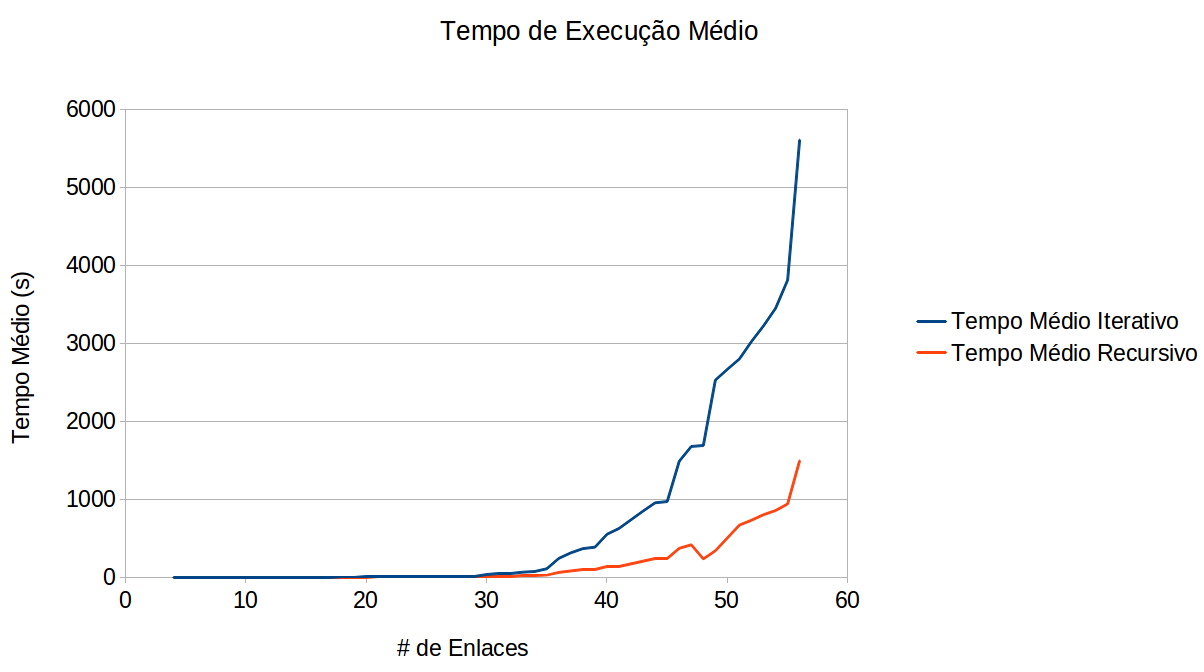
\includegraphics[width=1\linewidth]{figs/tempo128.png} 
    \caption{$n=128$} 
    \vspace{4ex}
  \end{minipage} 
\end{figure}

O primeiro fato a ser notado é que o algoritmo recursivo obteve menores tempos de execução para todos os valores de n. Isso reflete a menor complexidade de tempo teórica que algoritmo RECURSIVO tem em comparção com o algoritmo ITERATIVO. Em ambos os algoritmos, com o aumento de n, suas curvas se aproximam cada vez mais de uma exponencial, confirmando suas complexidades computacionais.

\section{Conclusão}

Nesse capítulo, a redução da complexidade computacional de O(m) para O(n) em algoritmos que iteram sobre os enlaces de um conjunto foi justificado através de técnicas de otimização. Em seguida, foi descrito um panorama sobre as técnicas de implementação e ambiente utilizados. 

Finalmente, usou-se o resultado das simulações para entender qual o impacto das complexidades computacionais teóricas quando os algoritmos são utilizados na prática. Além disso, também foi possível verificar o tamanho de |F| em função de m, que permitiu concluir a superioridade dos algoritmos aqui apresentados em relação aos algoritmos ingênuos e baseados em força bruta.

	\chapter{Conclusões e Trabalhos Futuros}
\label{cap:conclusoes}

\section{Conclusões}

A corretude dos algoritmos discutida nos Capítulos \ref{cap:iterativo} e \ref{cap:recursivo} garante que eles conseguem efetivamente enumerar todos os conjuntos de enlaces viáveis em uma rede. Sua complexidade computacional teórica também é analisada nesses capítulos e sua comprovação é observada nos resultados experimentais do Capítilo \ref{cap:resultados}. Observou-se que tais algoritmos terminam sua computação em tempo praticável para a aplicação motivadora deste trabalho. 

As redes usadas como entrada dos algoritmos são limitadas a no máximo 64 enlaces e isso pode reduzir o raio de aplicação dos algoritmos. Além disso, as complexidades computacionais teóricas foram aproximadas para redes de até 128 nós. Não é possível afirmar que o modelo usado para descrever a variação do número de conjuntos viáveis continua válido para redes com mais nós.

Portanto, conclui-se que o problema de enumeração de conjuntos viáveis pode ser resolvido usando os algoritmos propostos e, com isso, o objetivo do trabalho é alcançado.

\section{Trabalhos Futuros}

Como mencionado na seção anterior, ainda existem algumas limitações para o contexto de aplicação dos algoritmos. Na forma de proposta de trabalhos futuro, algumas ideias para reduzir tais limitações são apresentadas.

\subsection{Paralelização dos Algoritmos}

Os dois algoritmos apresentados são sequenciais. Por isso, é intuitivo pensar que melhores tempos de execução podem ser alcançados paralelizando-os. 

\subsubsection{Algoritmo Iterativo Paralelo}

Para o algoritmo ITERATIVO, a ideia é dividir a contagem. Existem $m$ ramos principais, uma para cada enlace da rede, que partem da raiz da árvore de combinações. Cada ramo principal possui $2^i$ vértices na árvore, onde $i$ é o índice do enlace $e_i$ que define a raiz desse ramo. 

Cada ramo é atribuído a uma das $T$ threads disponíveis. Mesmo que $T < m$, os $T$ primeiros ramos são alocados nas $T$ threads e, a medida que as threads terminam a contagem no ramo, elas passam para o próximo ramo $T+1, T+2, ..., m$. É importante manter a divisão dos m ramos principais para garantir que os saltos em uma porção da contagem não se sobreponham a outras porções.

A Figura \ref{fig:saltos} será usada para exemplificar o paralelismo. Em um dado ambiente computacional existem $T=3$ threads disponíveis. Como descrito, cada ramo principal da árvore será tratado por uma thread. Inicialmente, a thread $t_1$ cuidará do ramo $\{1\}$, a thread $t_2$ cuidará do ramo $\{2, 3\}$ e a thread $t_3$ cuidará do ramo $\{4, 5, 6, 7\}$. Assim que uma das threads terminar sua computação inicial ela assumirá o próximo ramo. 

Por exemplo, se $t_1$ acabar sua computação primeiro, ela cuidará do ramo $\{8,9,10,11,12,13,14,15\}$. Qualquer salto que saia de um ramo para o outro, resulta no término da thread, que será atribuída para outro ramo ainda não coberto, se houver. Por exemplo, nessa figura, a thread $t_3$ está cuidando do ramo com raiz em 4, que não é viável. Normalmente, um salto seria dado de 4 para 8, que é o pai do último ramo principal. Contudo, como $t_1$ acaba antes de $t_3$, $t_1$ já está cuidando desse ramo e, portanto, $t_3$ simplesmente encerra sua computação.  
 
\subsubsection{Algoritmo Recursivo Paralelo}

Uma abordagem semelhante seria adotada para o algoritmo RECURSIVO. Nesse algoritmo, sua primeira execução, ou seja, quando B=0, é diferenciada das demais. O tratamento para o caso em que B=0 é chamar RECURSIVO para todos os m filhos de 0 na árvore de combinações, ou seja, as raizes dos ramos principais. Logo, basta que a iteração sobre os filhos de 0 seja paralelizada de maneira análoga ao caso do algoritmo ITERATIVO. 

\subsection{Teste de Máscaras}

Seja $C$ um vértice de uma árvore de cobinações. Se $C$ não é viável, então se os enlaces do conjunto $C$ também aparecerem em outro conjunto $C'$, $C'$ também não é viável. A prova para esse fato é anóloga à justficativa da propriedade de Inviabilidade Hereditária apresentada no Capítulo \ref{cap:modelagem}.

Seja $B$ um número inteiro que codifica o conjunto $C$ não viável. Seja $\{b_{m-1}, b_{m-2}, ..., b_1, b_0\}$ a sequência dos bits de $B$ que representam a pertinência dos enlaces de $E(G)$ em $C$. Os bits ativos em $B$ formam um padrão, de forma que, qualquer número inteiro $B'$ que contenha esse padrão também não é viável.

A ideia do Teste de Máscara é, uma vez que um conjunto não viável é encontrado, seu valor codificado $B$ é adicionado a uma lista de máscaras. Sempre que a viabilidade de outros conjuntos forem testadas, tenta-se encontrar o padrão de bits de todos os números na lista de máscaras. Se o padrão de pelo menos uma máscara for encontrado no número que codifica o conjunto testado, então tal conjunto também não é viável. Por exemplo, se $(3)_{10} = (0011)_2$ não for viável, então certamente $(7)_{10} = (0111)_2$, $(11)_{10} = (1011)_2$ e $(15)_{10} = (1111)_2$ também não serão.

O teste para checar se o padrão de $B$ está contido em $B'$ pode ser feito por uma simples operação bit-a-bit. Contudo, se há muitos conjuntos não viáveis em uma rede, a complexidade de tempo para esse teste pode aumentar muito. Por isso, a melhor estratégia para implementar o Teste de Máscaras é fazê-lo em paralelo ao teste de viabilidade.

\subsection{Aumentar Redes}

O limitante mais grave dos algoritmos apresentados é o fato de só funcionarem para redes de até 64 enlaces. Essa limitação surge devido as arquiteturas dos computadores atuais serem de, no máximo, 64 bits. Por isso, em qualquer linguagem de programação, o maior inteiro que se pode ter é $2^{64}-1$. Logo, como os algoritmos baseiam-se em números inteiros que representam os conjuntos de enlaces, apenas $2^{64}-1$ conjuntos de enlaces pode ser testado.

Contudo, existem bibliotecas que oferecem manipulação numérica para inteiros maiores que 64 bits. Para C++, a biblioteca XXX oferece uma classe que permite representar inteiros até 128 bem como as operações matemáticas básicas, que são suficientes para escrever os algoritmos. Apesar de existir recursos para isso, ao fazer a adaptação para um cenário em que 128 enlaces são permitidos, novas complexidades devem ser analisadas para verificar se a aplicabilidade dos algoritmos se mantém.

	
  \backmatter
  \bibliographystyle{coppetex/coppe-unsrt}
  \bibliography{projeto}
\end{document}
